\appendix

\chapter{Additional Figures}

\section{Chapter 3 Additional Figures}

\subsection{MC-LP Order} \label{section:appendix:params_p2}

%\textbf{p2 = L / (M-1)  (MINT based on RIR length)}

\begin{figure}[H]
	\centering
	\begin{subfigure}[b]{0.32\textwidth}
		\centering
		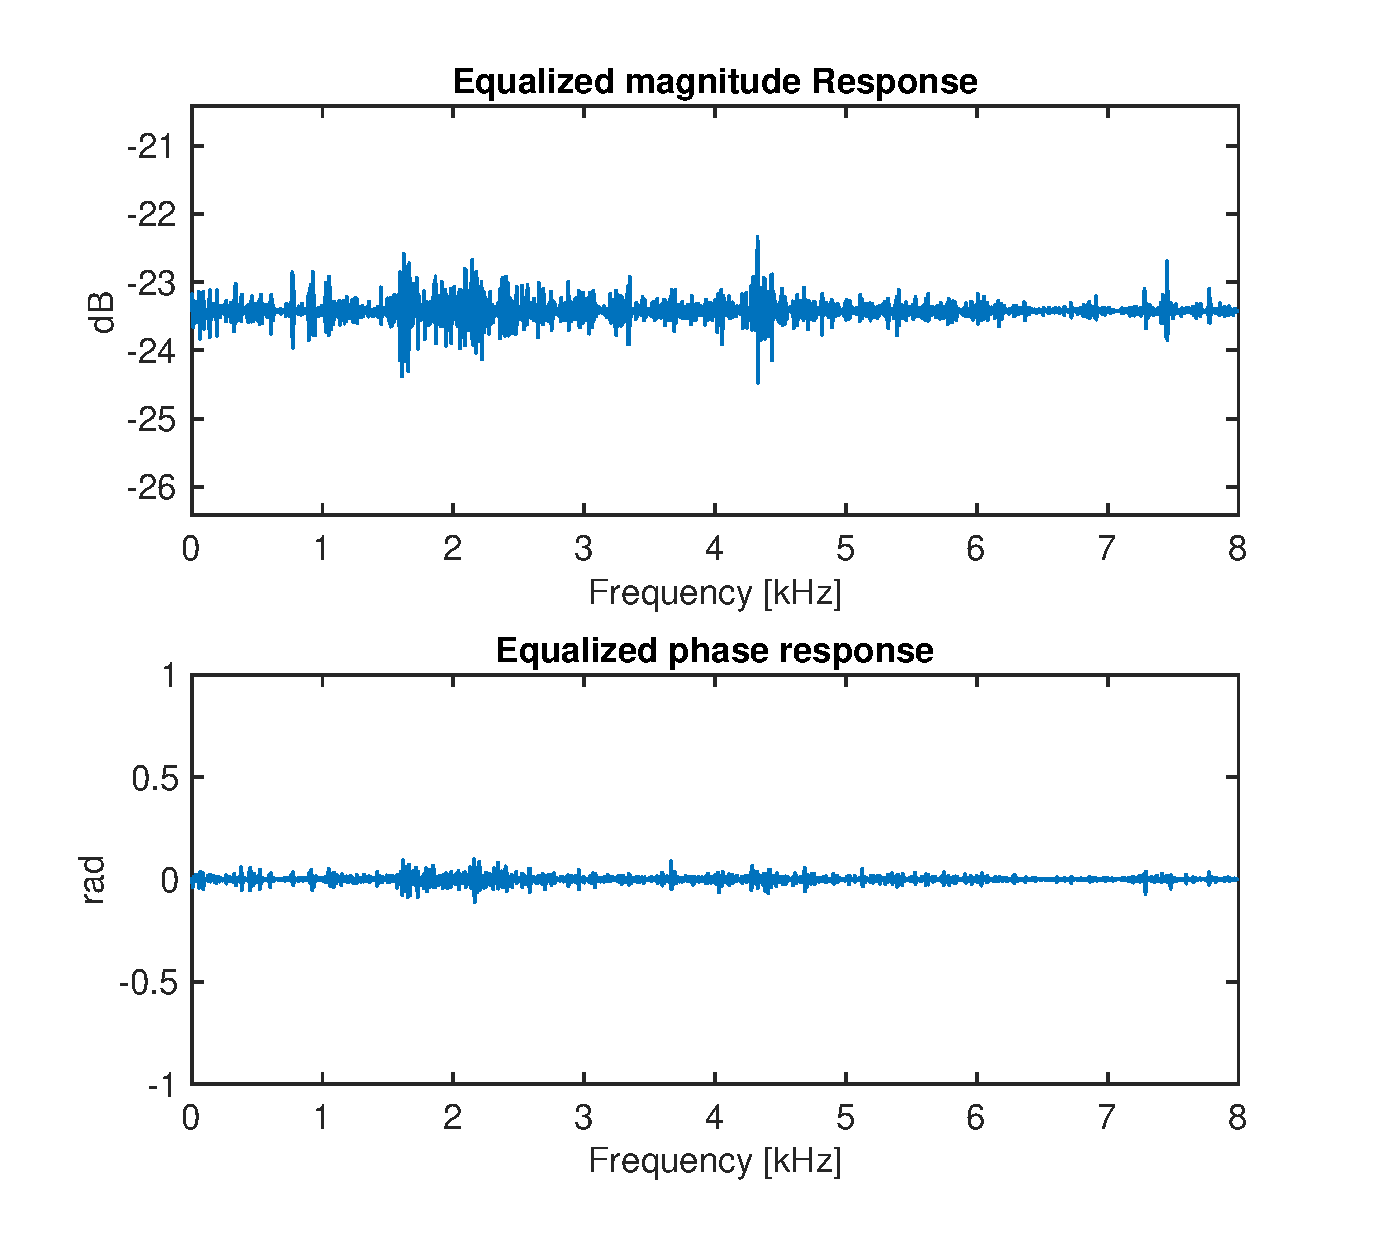
\includegraphics[width=\textwidth]{Equalized_RTF_L_div_M_minus_1}
		\subcaption{test} \label{subfig:test_subfig_1}
	\end{subfigure}
	\hfill
	\begin{subfigure}[b]{0.32\textwidth}
		\centering
		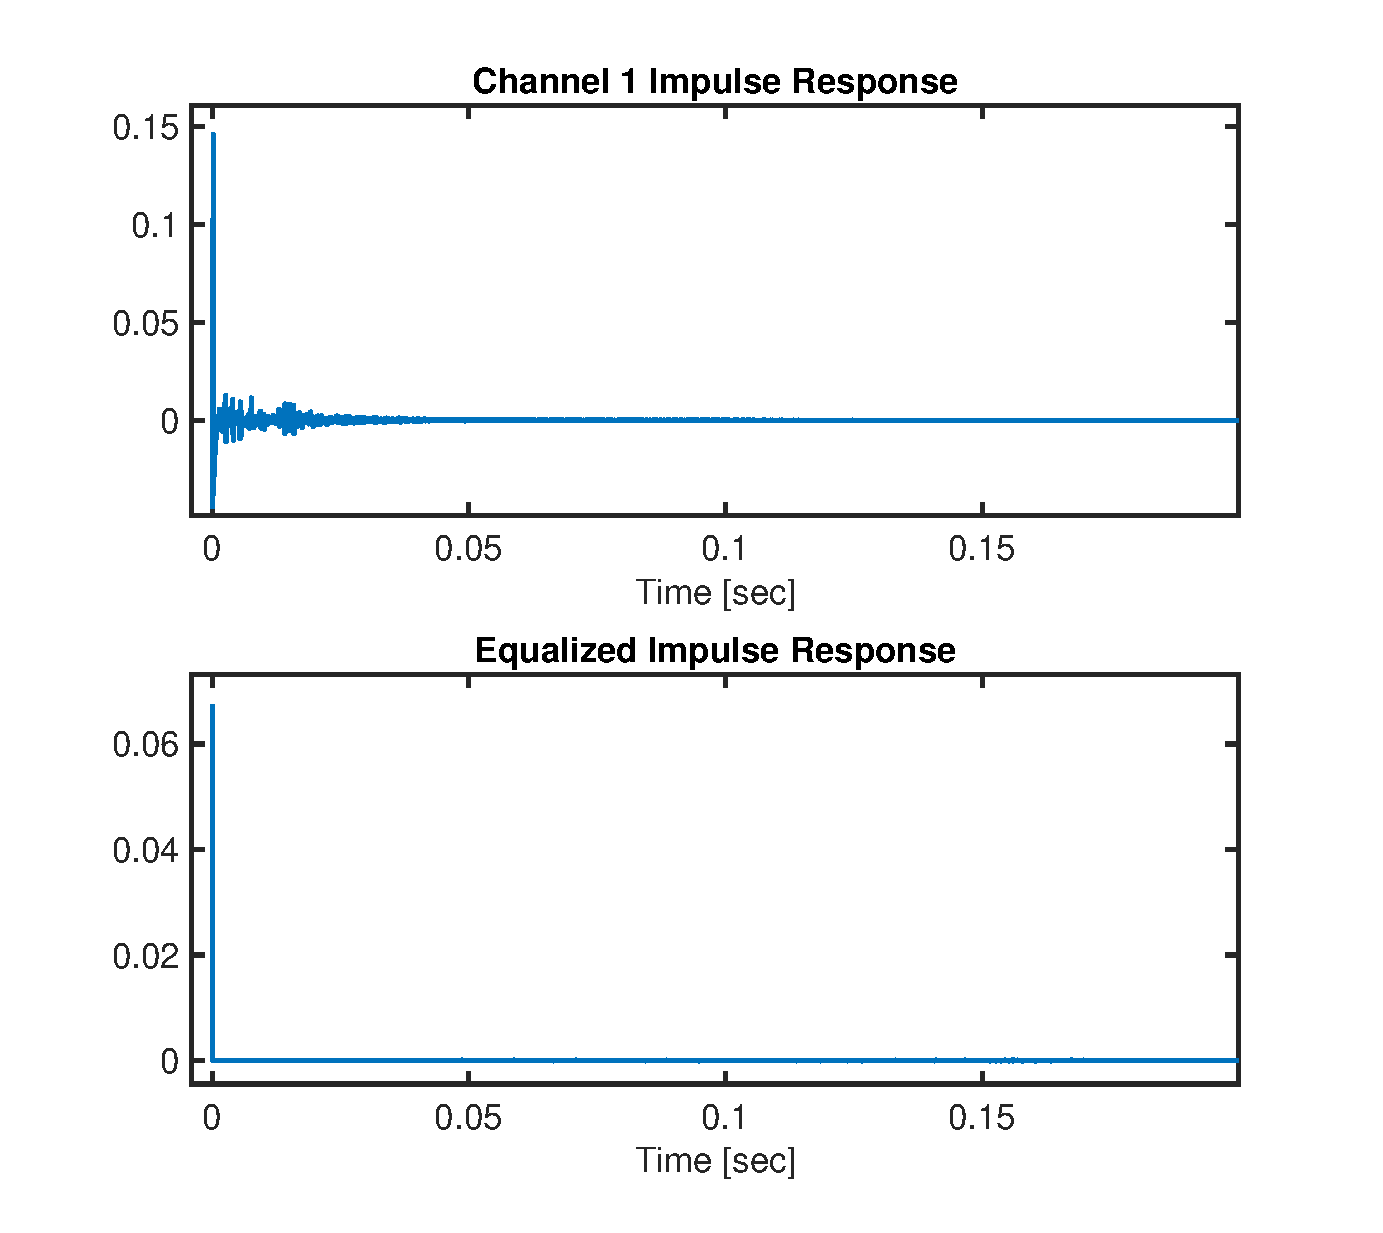
\includegraphics[width=\textwidth]{EIR_L_div_M_minus_1}
	\end{subfigure}
	\hfill
	\begin{subfigure}[b]{0.32\textwidth}
		\centering
		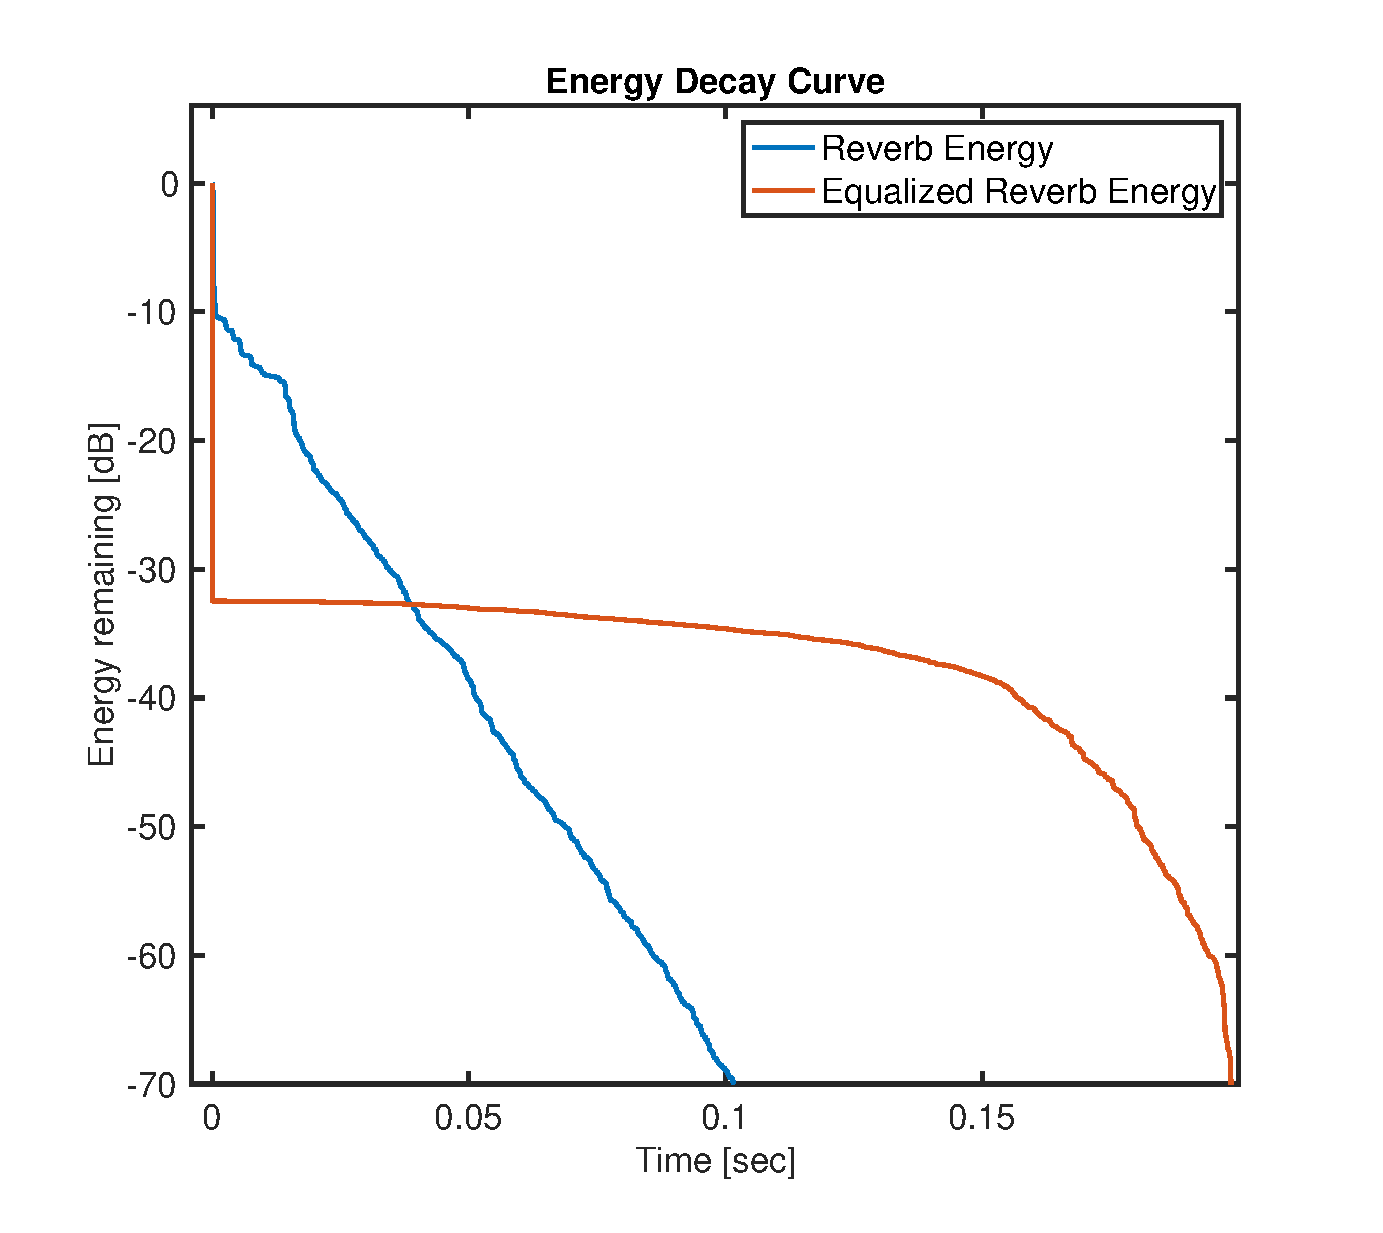
\includegraphics[width=\textwidth]{EDC_L_div_M_minus_1}
	\end{subfigure}
	\hfill
	\caption[Detailed behaviour of DAP with $p_2 = L/\left(M-1\right)$]{Delay-and-Predict dereverberation performance with multichannel linear prediction order $\mathrm{p2} = L / (M-1)$, where $L$ is the FIR RIR length and $M$ is the number of channels. Figure \ref{fig:params_p2_stage1} shows the common source whitening filter used.}
	\label{fig:params_p2_L}
\end{figure}

%\textbf{p2 = N60 / (M-1)  (MINT based on T60)}

\begin{figure}[H]
	\centering
	%\begin{subfigure}[b]{0.49\textwidth}
	%	\centering
	%	\includegraphics[width=\textwidth]{S1_N60_div_M_minus_1}
	%\end{subfigure}
	%\hfill
	\begin{subfigure}[b]{0.32\textwidth}
		\centering
		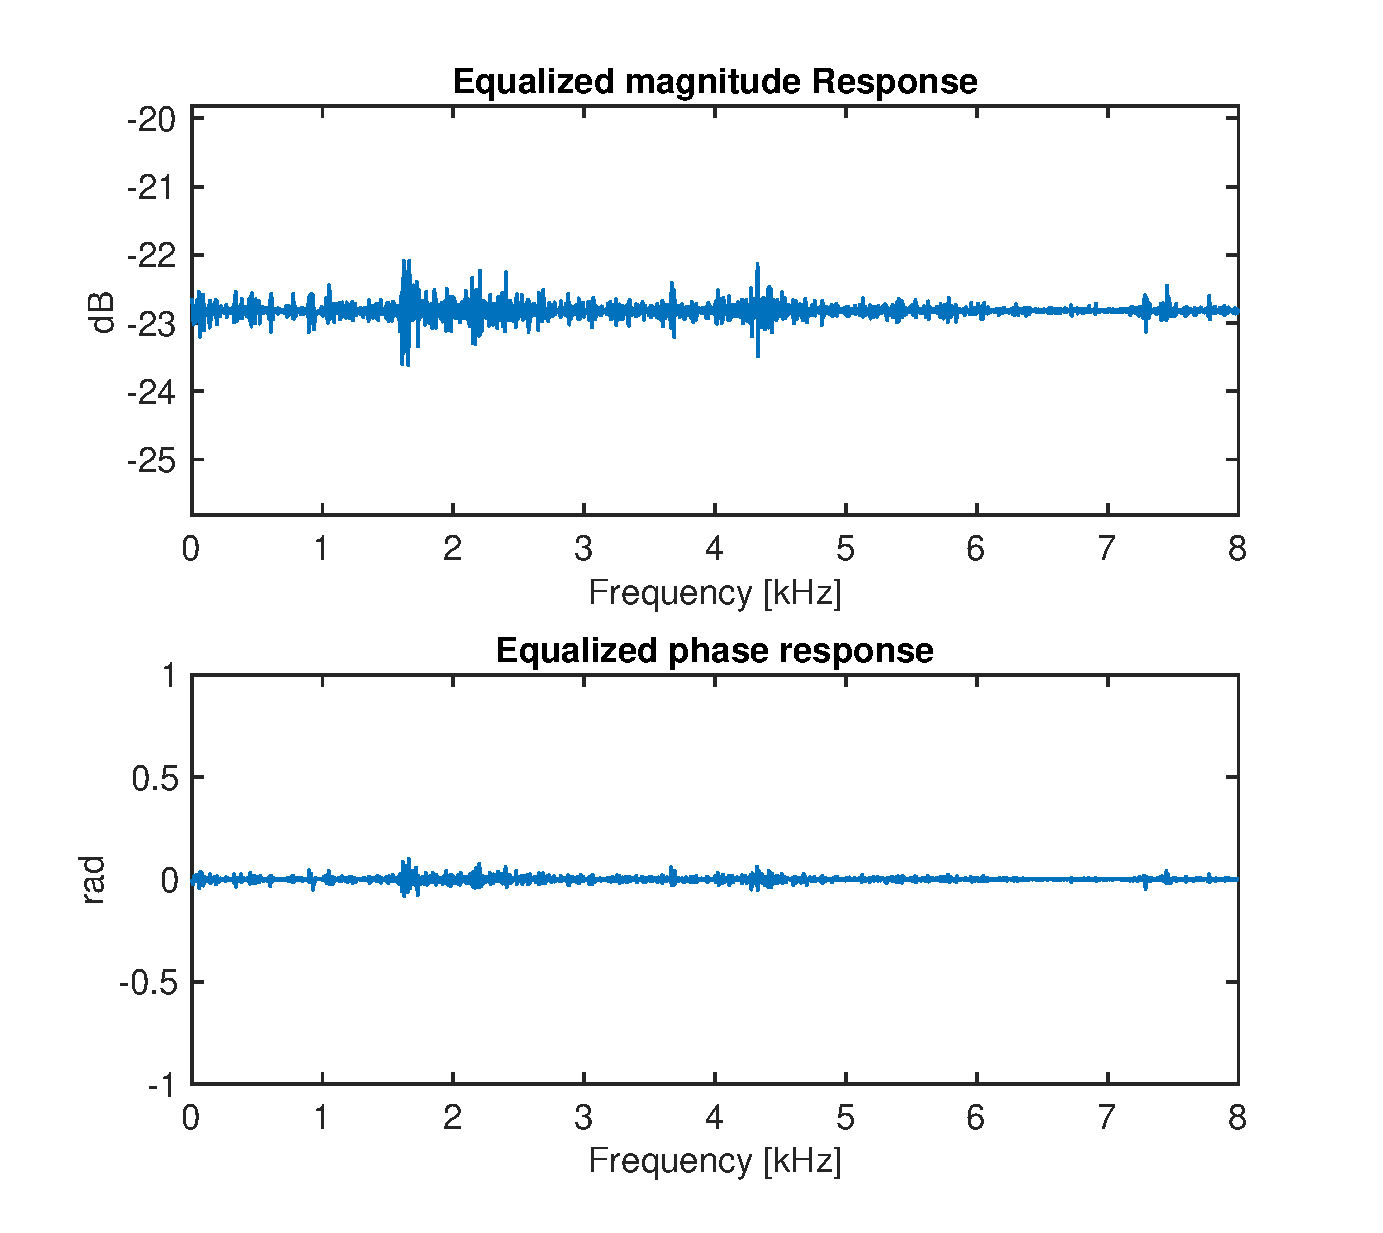
\includegraphics[width=\textwidth]{Equalized_RTF_N60_div_M_minus_1}
	\end{subfigure}
	\hfill
	\begin{subfigure}[b]{0.32\textwidth}
		\centering
		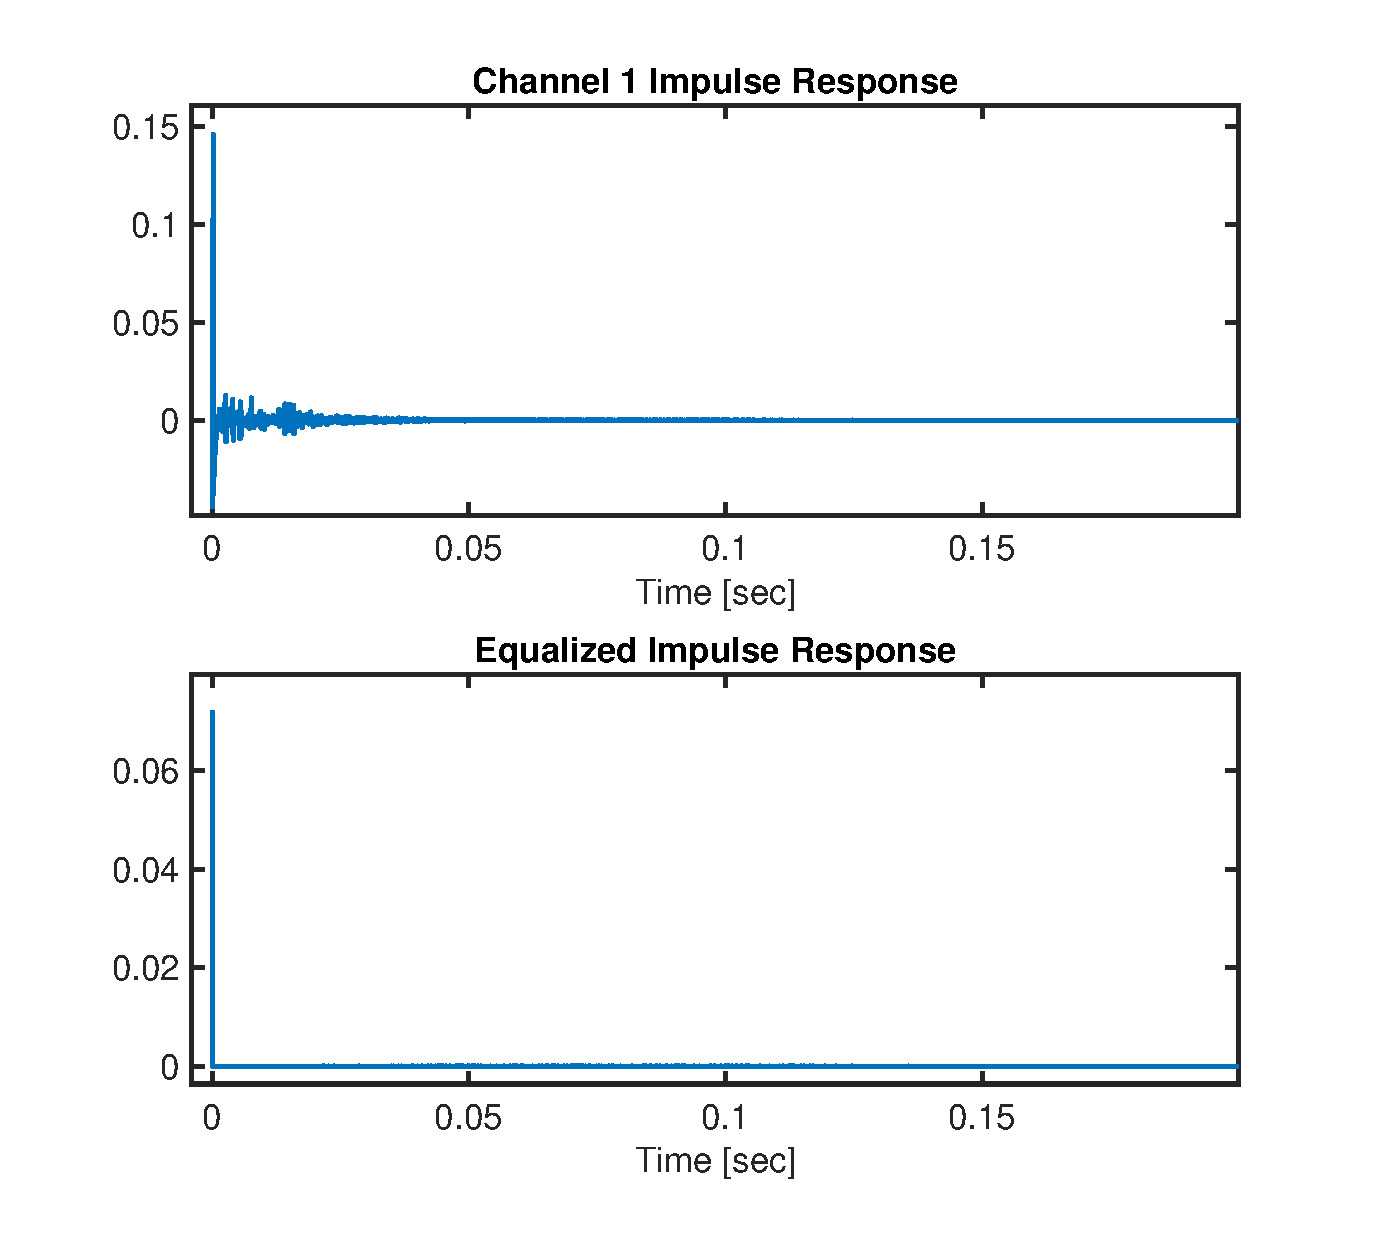
\includegraphics[width=\textwidth]{EIR_N60_div_M_minus_1}
	\end{subfigure}
	\hfill
	\begin{subfigure}[b]{0.32\textwidth}
		\centering
		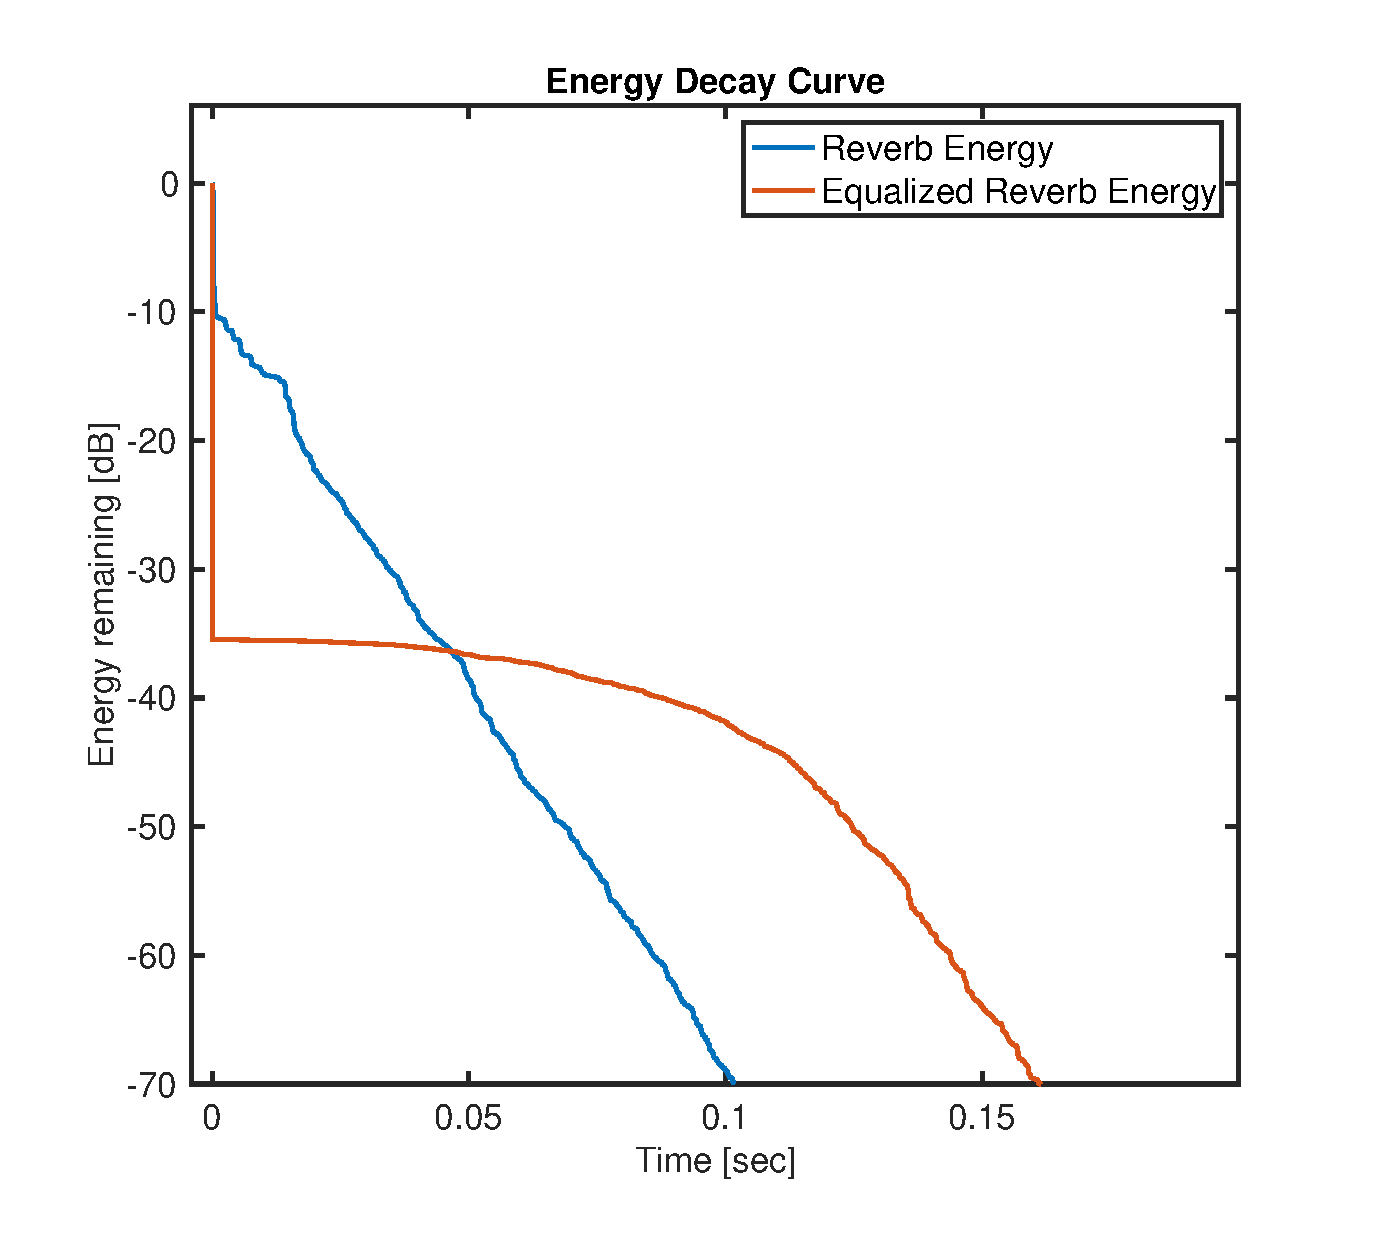
\includegraphics[width=\textwidth]{EDC_N60_div_M_minus_1}
	\end{subfigure}
	\hfill
	\caption[Detailed behaviour of DAP with $p_2 = N60/\left(M-1\right)$]{Delay-and-Predict dereverberation performance with multichannel linear prediction order $\mathrm{p2} = \mathrm{N60} / (M-1)$, where N60 is the number of samples corresponding to the T60 and $M$ is the number of channels (i.e., the MINT condition based on T60 rather than the FIR RIR length). Figure \ref{fig:params_p2_stage1} shows the common source whitening filter used.}
	\label{fig:params_p2_N60}
\end{figure}

%\textbf{p2 = 0p75 * N60 / (M-1) (Suboptimal)}

\begin{figure}[H]
	\centering
	%\begin{subfigure}[b]{0.49\textwidth}
	%	\centering
	%	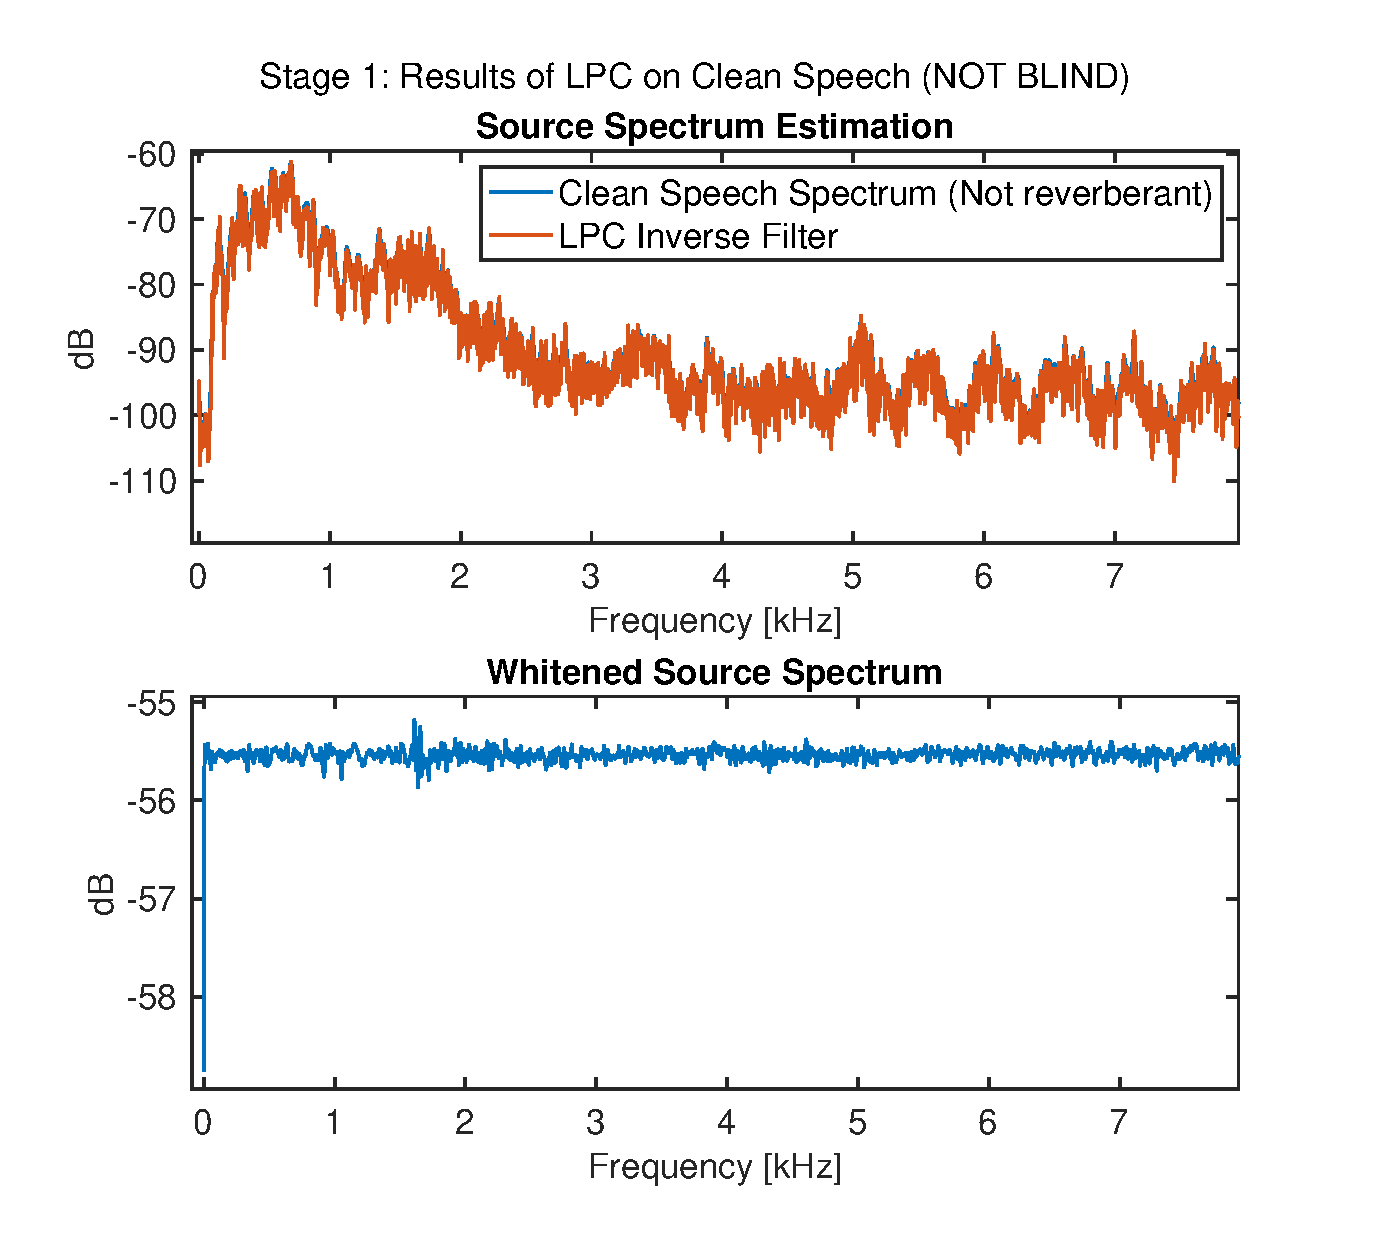
\includegraphics[width=\textwidth]{S1_0p75N60_div_M_minus_1}
	%\end{subfigure}
	%\hfill
	\begin{subfigure}[b]{0.32\textwidth}
		\centering
		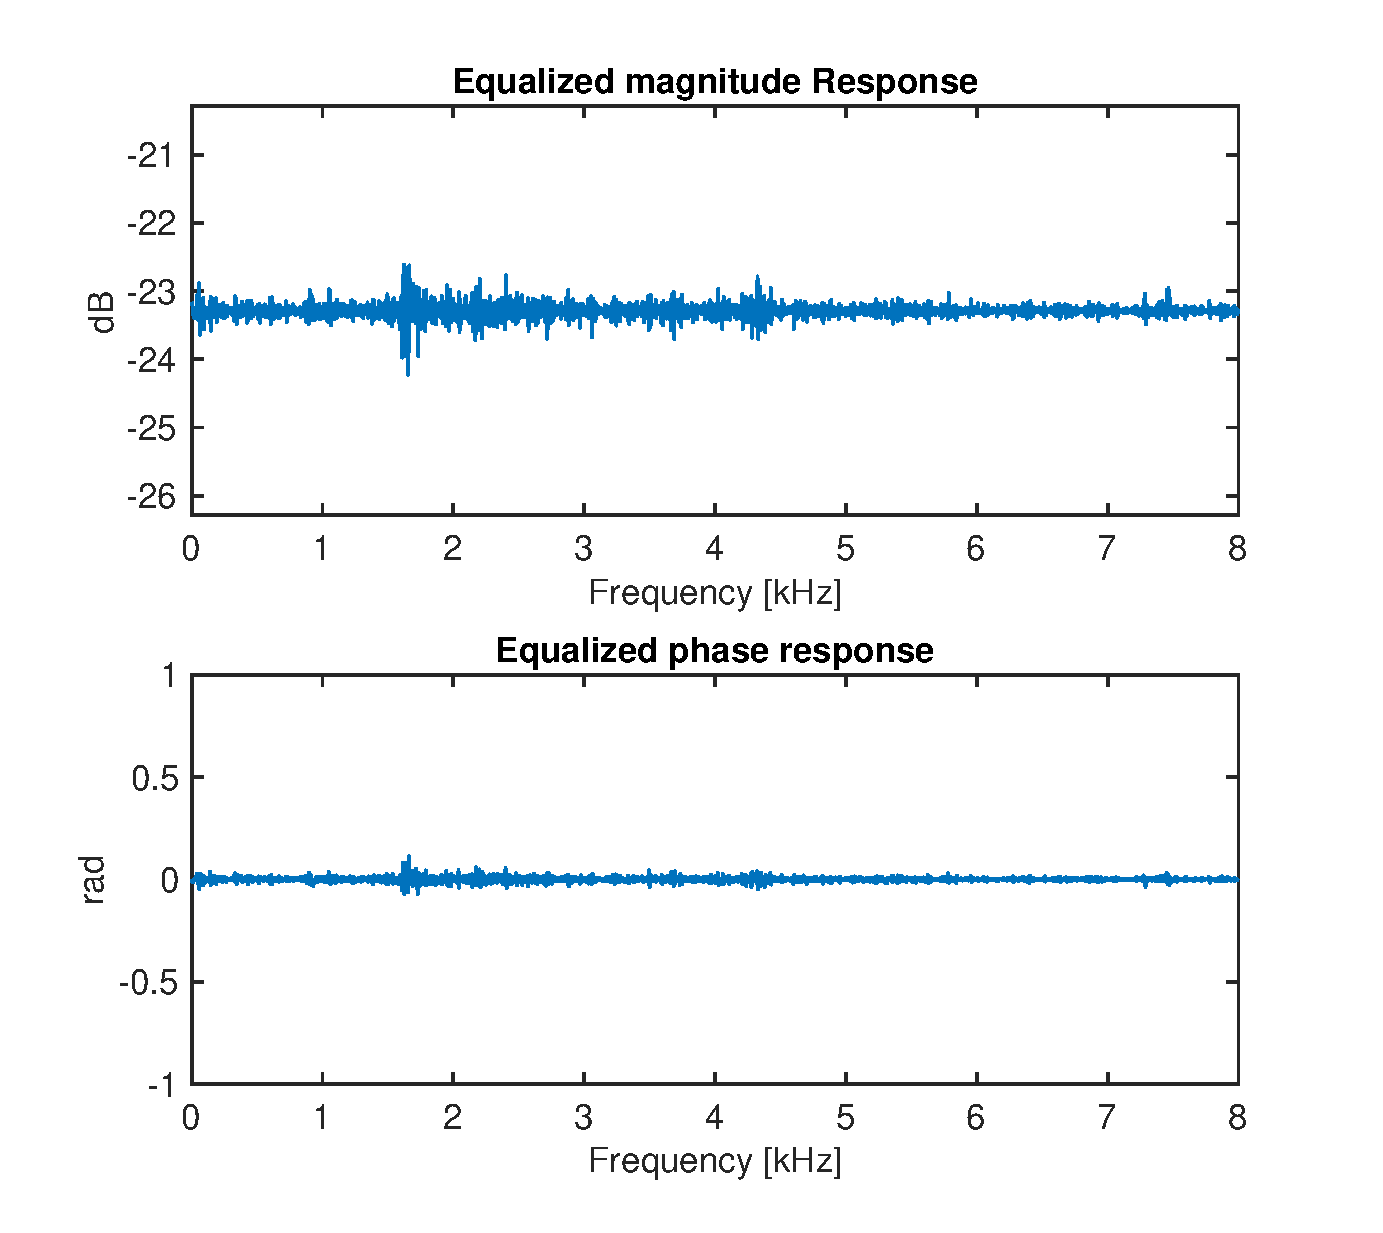
\includegraphics[width=\textwidth]{Equalized_RTF_0p75N60_div_M_minus_1}
	\end{subfigure}
	\hfill
	\begin{subfigure}[b]{0.32\textwidth}
		\centering
		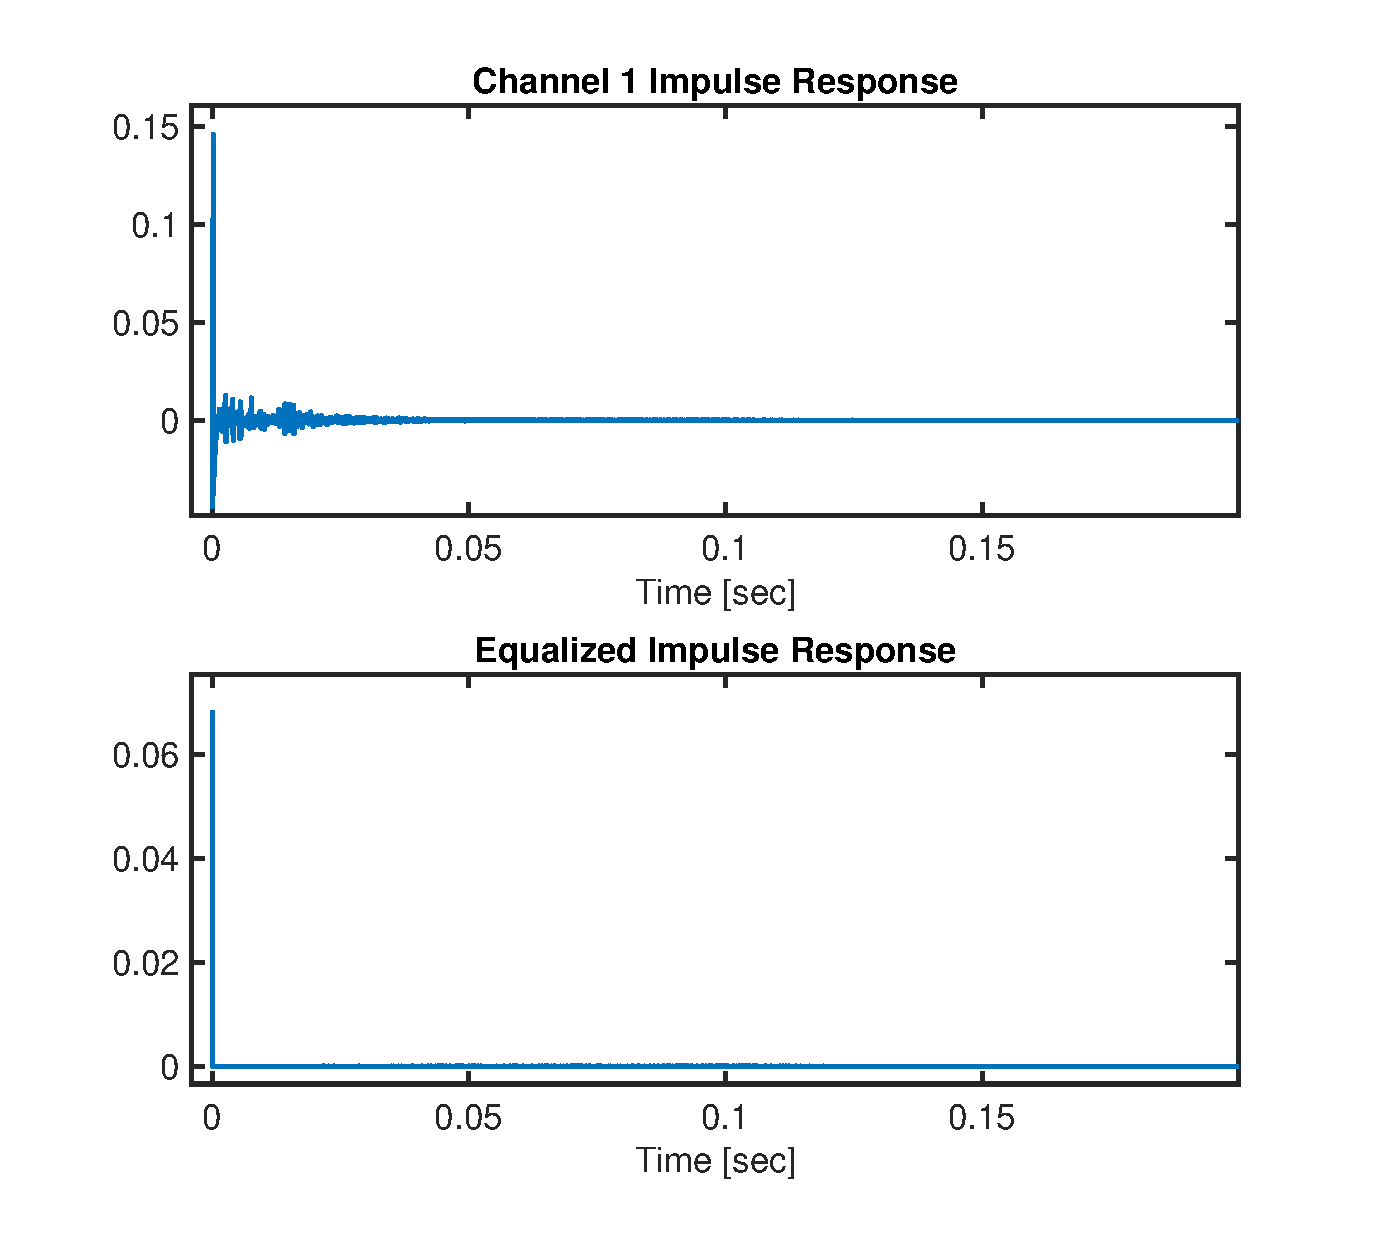
\includegraphics[width=\textwidth]{EIR_0p75N60_div_M_minus_1}
	\end{subfigure}
	\hfill
	\begin{subfigure}[b]{0.32\textwidth}
		\centering
		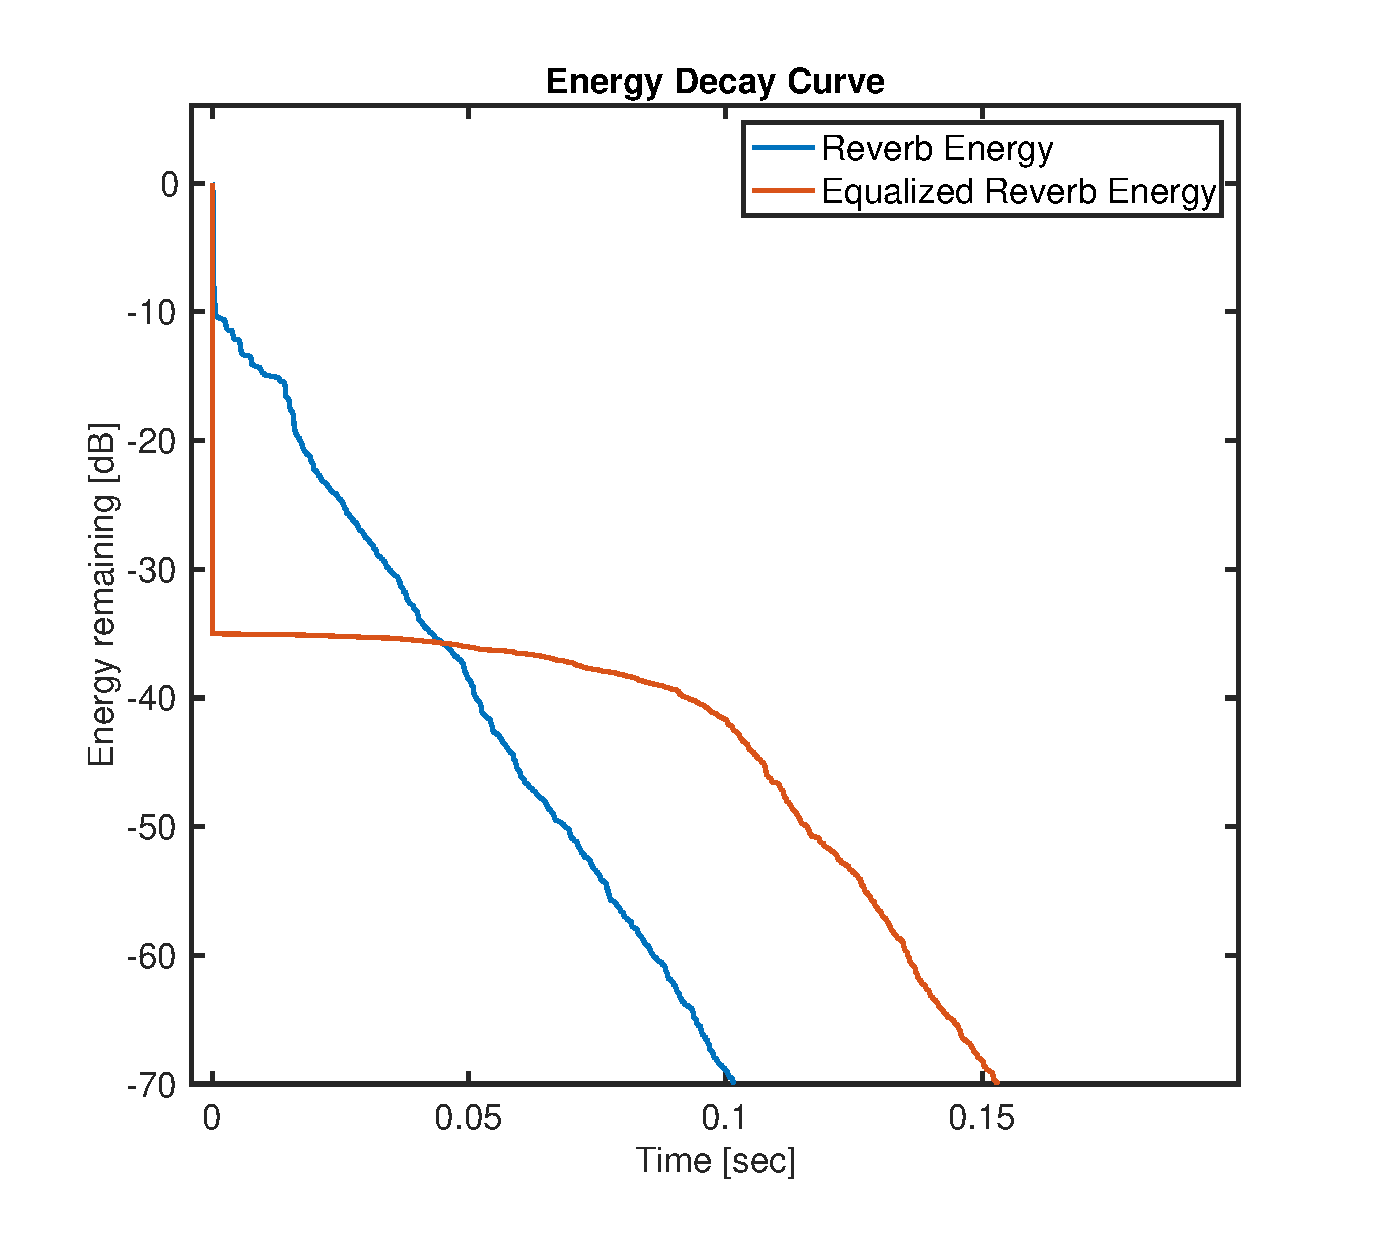
\includegraphics[width=\textwidth]{EDC_0p75N60_div_M_minus_1}
	\end{subfigure}
	\hfill
	\caption[Detailed behaviour of DAP with $p_2 = 0.75 \cdot N60/\left(M-1\right)$]{Delay-and-Predict dereverberation performance with multichannel linear prediction order $\mathrm{p2} = 0.75 \cdot \mathrm{N60} / (M-1)$, where N60 is the number of samples corresponding to the T60 and $M$ is the number of channels (i.e., suboptimal with respect to the MINT condition based on T60 rather than the FIR RIR length). Figure \ref{fig:params_p2_stage1} shows the common source whitening filter used.}
	\label{fig:params_p2_0p75_N60}
\end{figure}

%\textbf{p2 = 0.5 * N60 / (M-1) (More suboptimal)}

\begin{figure}[H]
	\centering
	%\begin{subfigure}[b]{0.49\textwidth}
	%	\centering
	%	\includegraphics[width=\textwidth]{S1_0p5N60_div_M_minus_1}
	%\end{subfigure}
	%\hfill
	\begin{subfigure}[b]{0.32\textwidth}
		\centering
		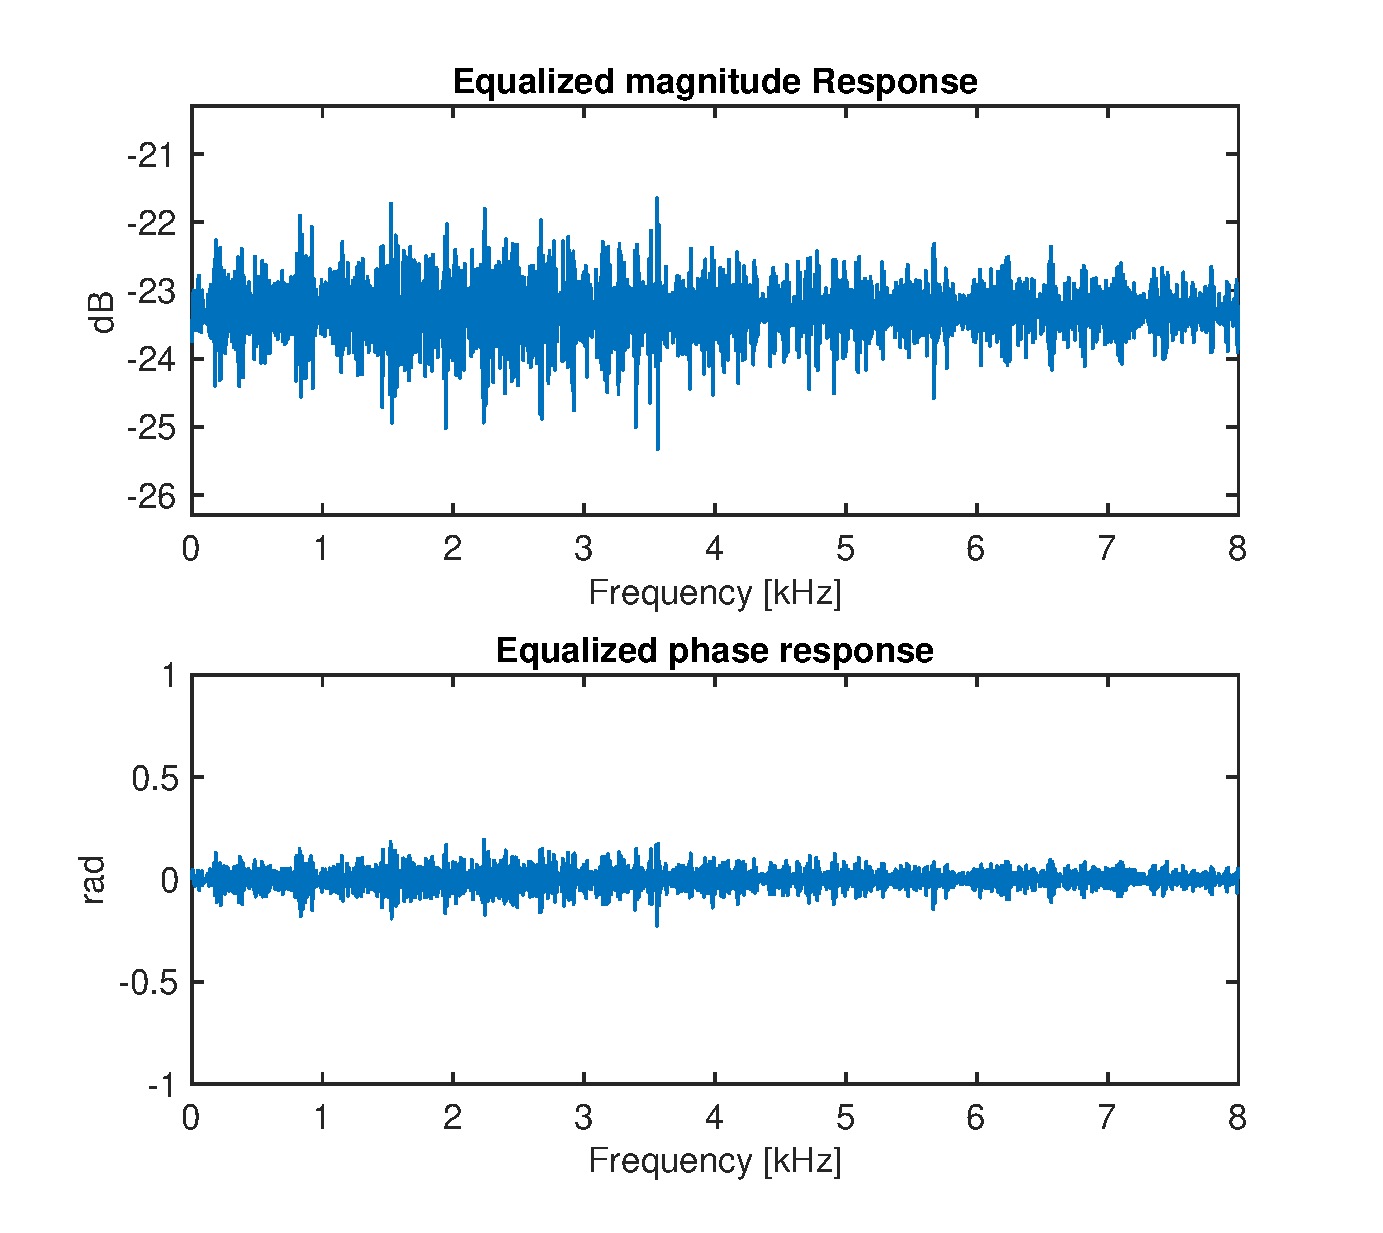
\includegraphics[width=\textwidth]{Equalized_RTF_0p5N60_div_M_minus_1}
	\end{subfigure}
	\hfill
	\begin{subfigure}[b]{0.32\textwidth}
		\centering
		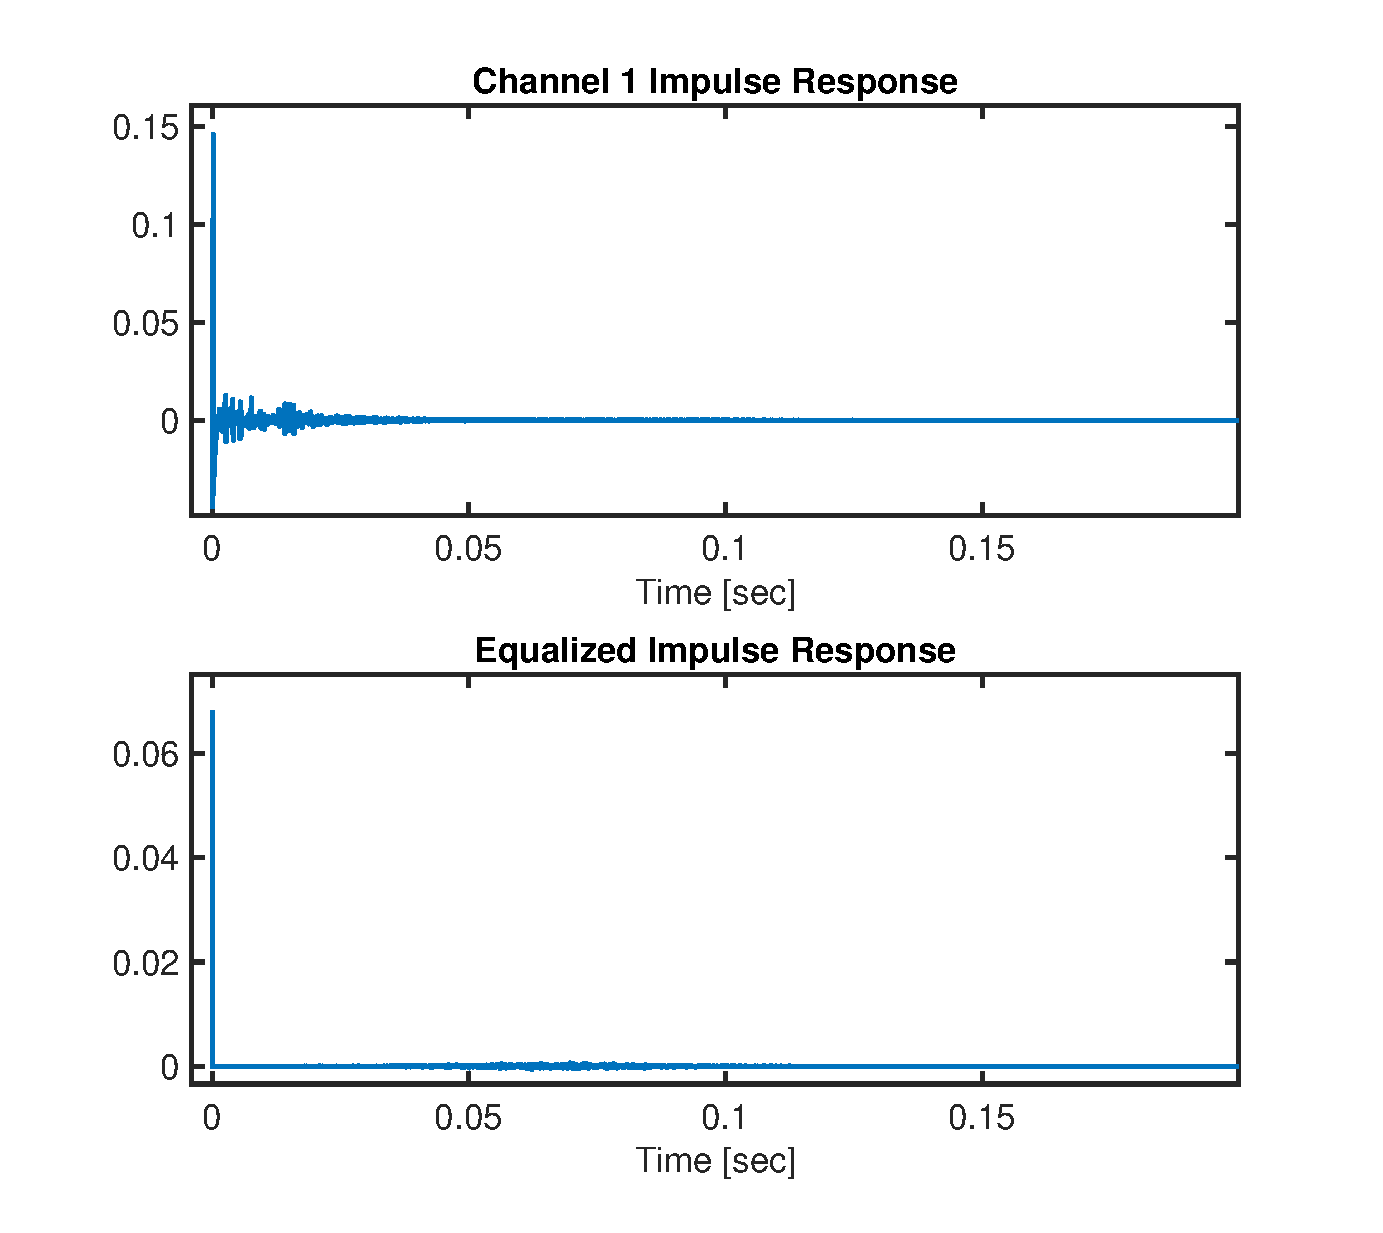
\includegraphics[width=\textwidth]{EIR_0p5N60_div_M_minus_1}
	\end{subfigure}
	\hfill
	\begin{subfigure}[b]{0.32\textwidth}
		\centering
		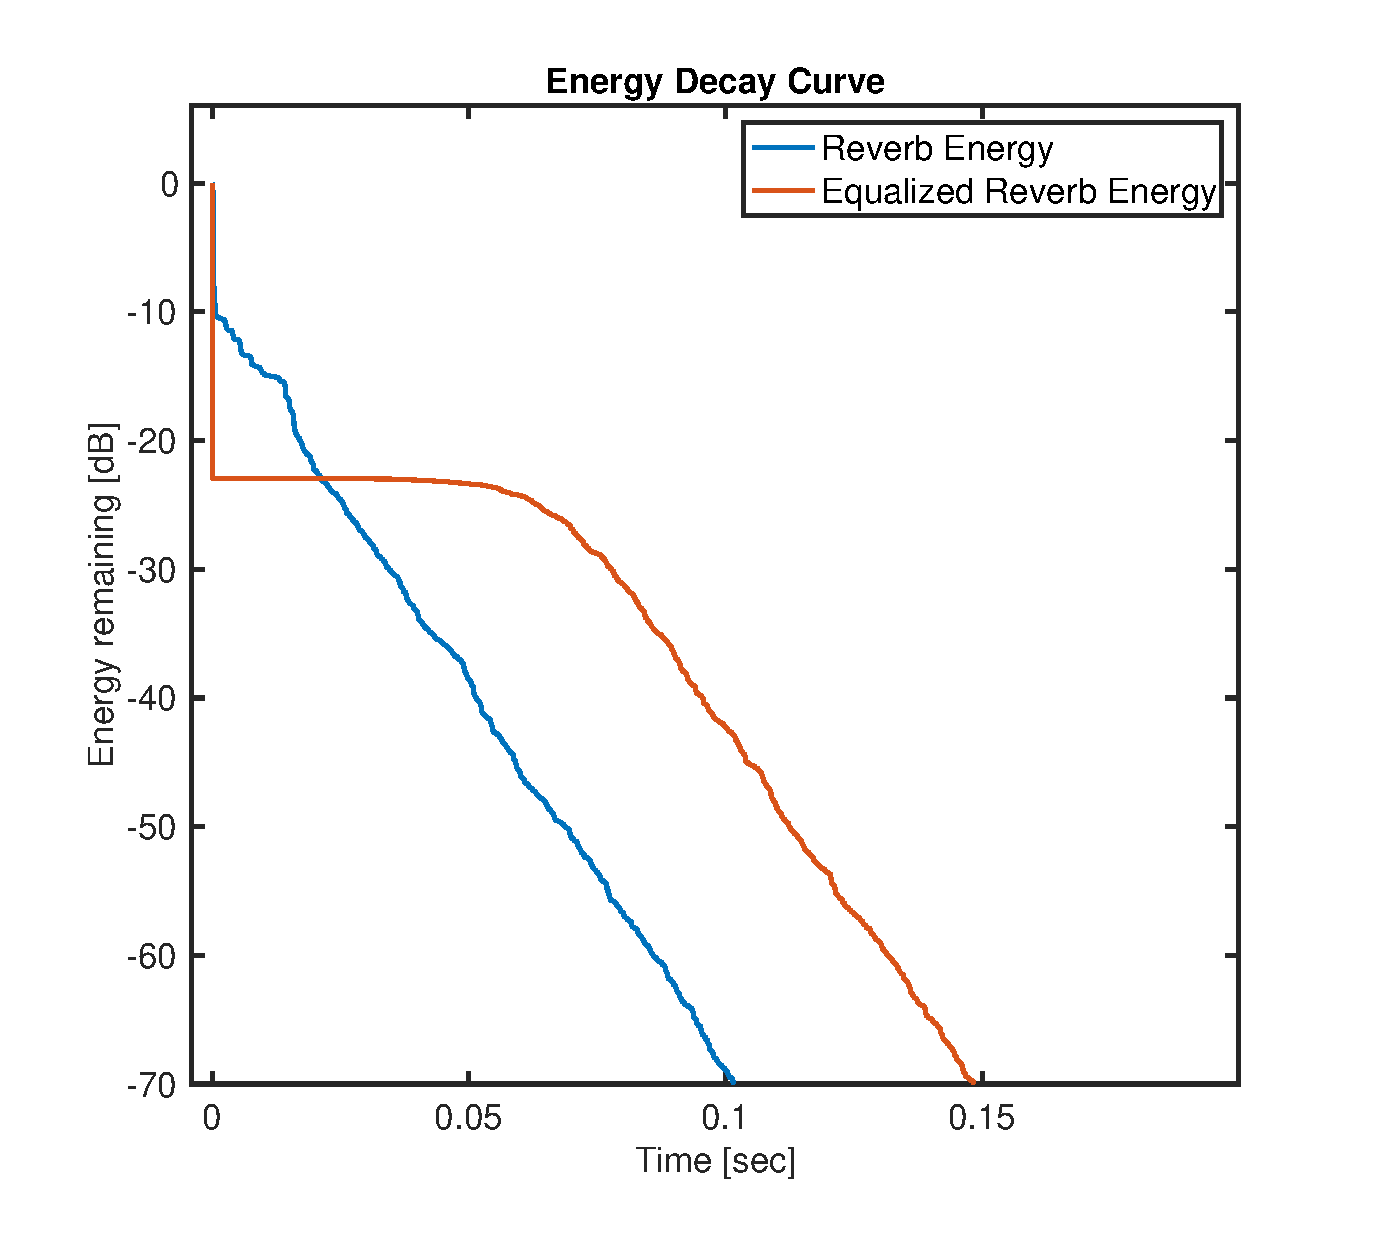
\includegraphics[width=\textwidth]{EDC_0p5N60_div_M_minus_1}
	\end{subfigure}
	\hfill
	\caption[Detailed behaviour of DAP with $p_2 = 0.5 \cdot N60/\left(M-1\right)$]{Delay-and-Predict dereverberation performance with multichannel linear prediction order $\mathrm{p2} = 0.5 \cdot \mathrm{N60} / (M-1)$, where N60 is the number of samples corresponding to the T60 and $M$ is the number of channels (i.e., More suboptimal with respect to the MINT condition based on T60 rather than the FIR RIR length). Figure \ref{fig:params_p2_stage1} shows the common source whitening filter used.}
	\label{fig:params_p2_0p5_N60}
\end{figure}

\subsection{Source Whitening Order} \label{section:appendix:params_p1}

%\textbf{p1 = 200 (Original Paper)}

\begin{figure}[H]
	\centering
	\begin{subfigure}[b]{0.49\textwidth}
		\centering
		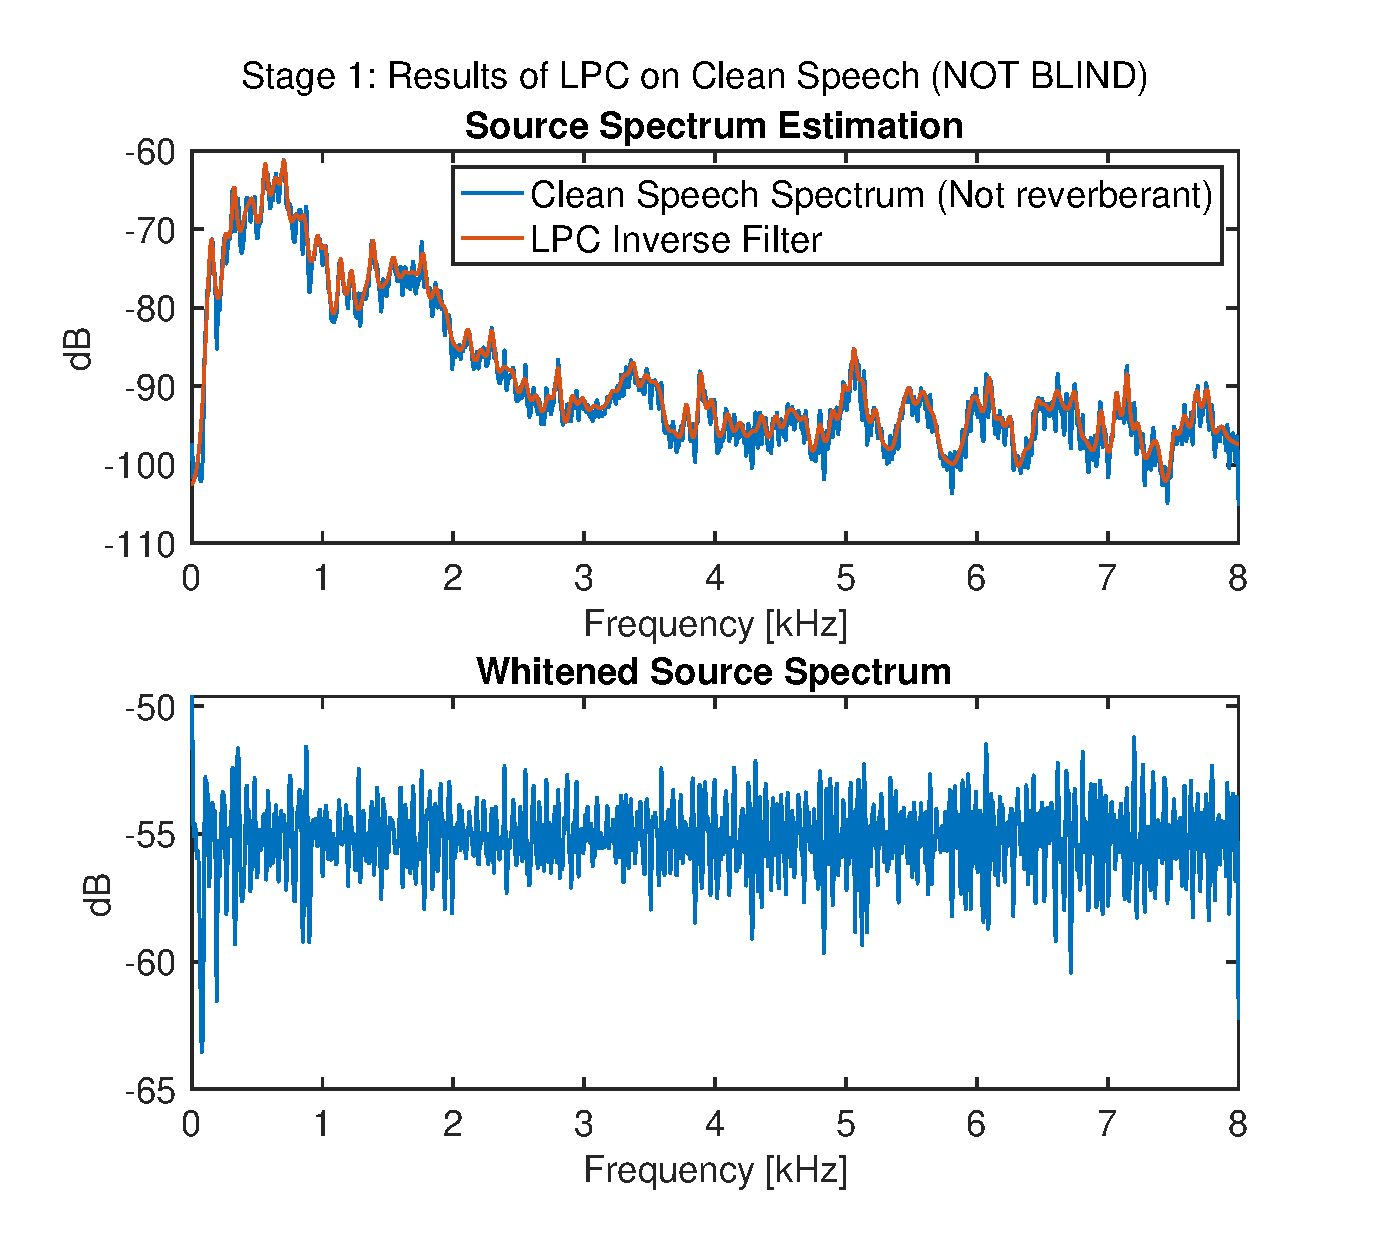
\includegraphics[width=\textwidth]{S1_p1_200}
	\end{subfigure}
	\hfill
	\begin{subfigure}[b]{0.49\textwidth}
		\centering
		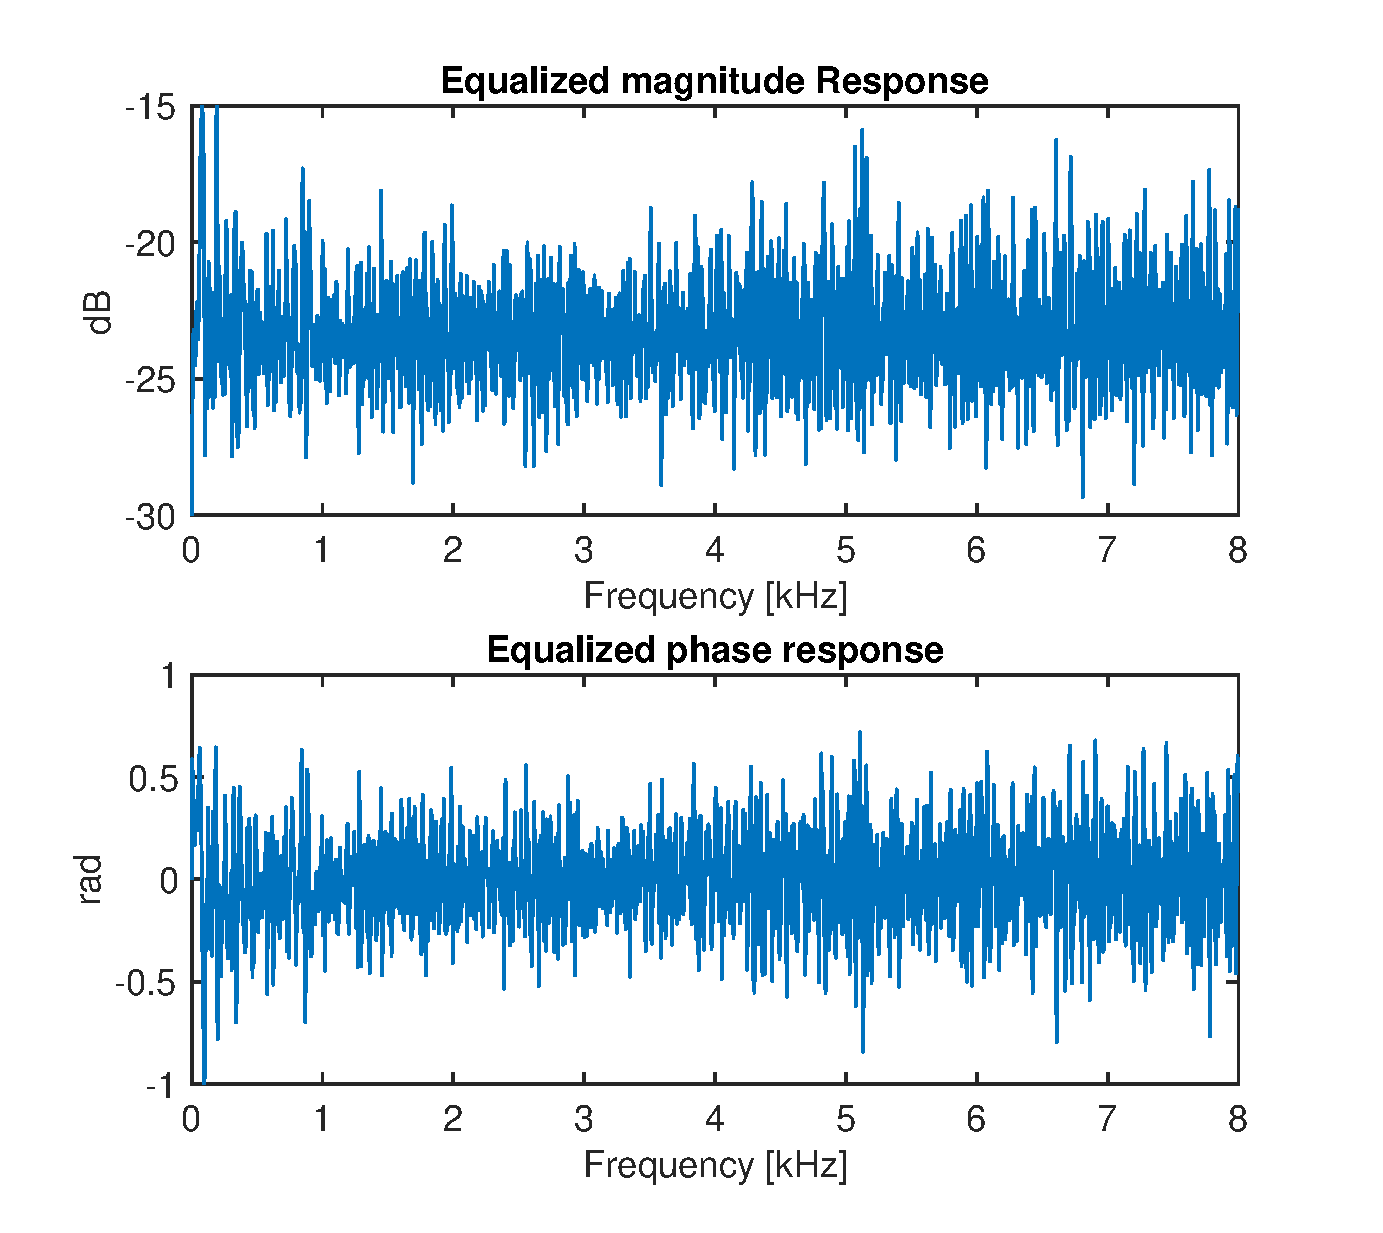
\includegraphics[width=\textwidth]{Equalized_RTF_p1_200}
	\end{subfigure}
	\hfill
	\begin{subfigure}[b]{0.49\textwidth}
		\centering
		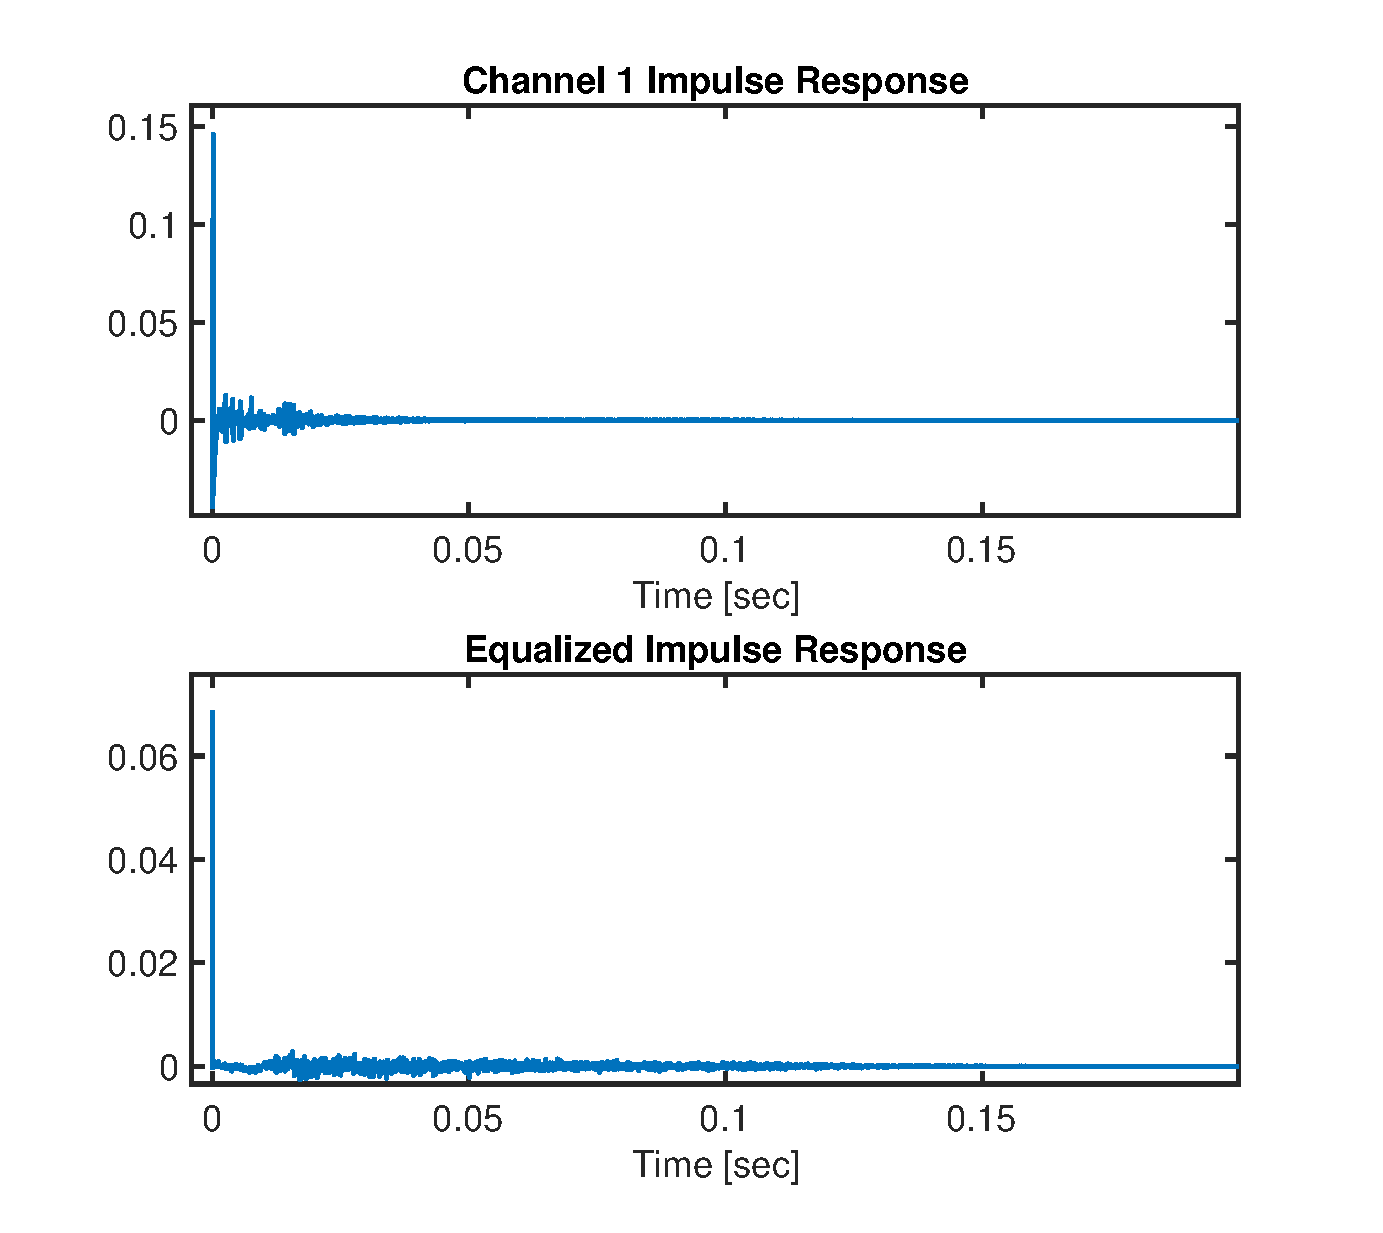
\includegraphics[width=\textwidth]{EIR_p1_200}
	\end{subfigure}
	\hfill
	\begin{subfigure}[b]{0.49\textwidth}
		\centering
		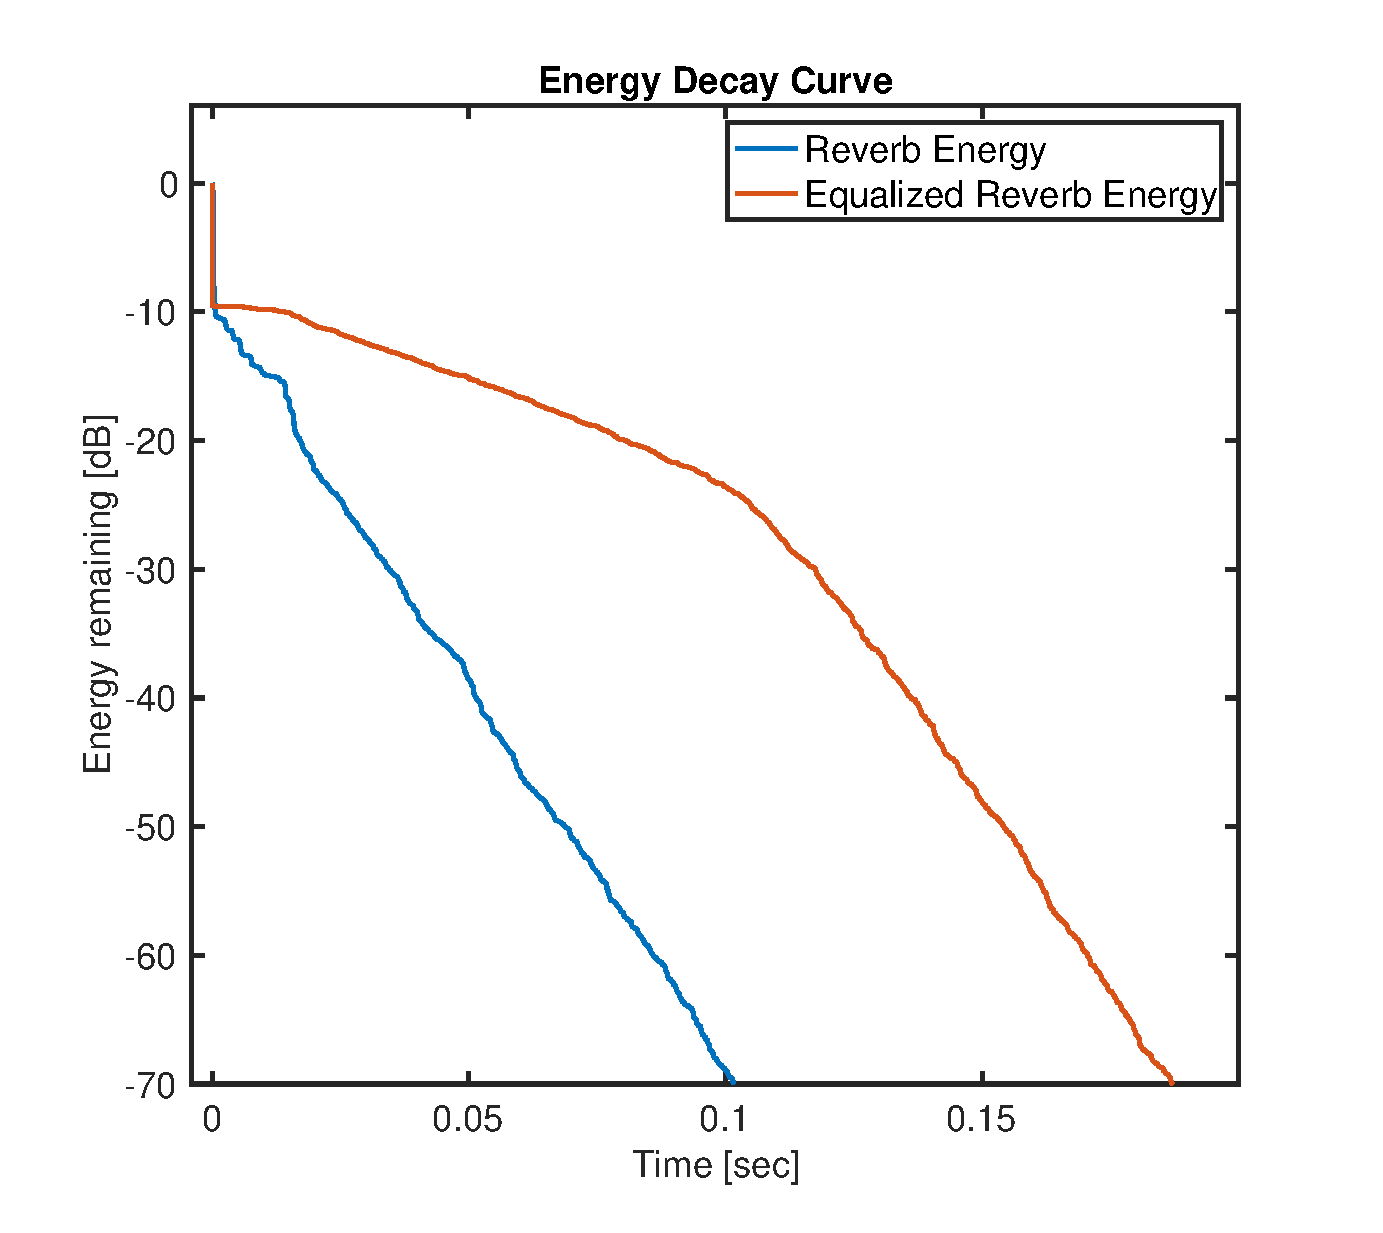
\includegraphics[width=\textwidth]{EDC_p1_200}
	\end{subfigure}
	\hfill
	\caption[Detailed behaviour of DAP with $p_1 = 200$]{Delay-and-Predict dereverberation performance with source whitening prediction order $\mathrm{p1} = 200$ and multichannel linear prediction order $\mathrm{p2} = \mathrm{N60}  / (M-1)$.}
	\label{fig:params_p1_200}
\end{figure}

%\textbf{p1 = 1000}

\begin{figure}[H]
	\centering
	\begin{subfigure}[b]{0.49\textwidth}
		\centering
		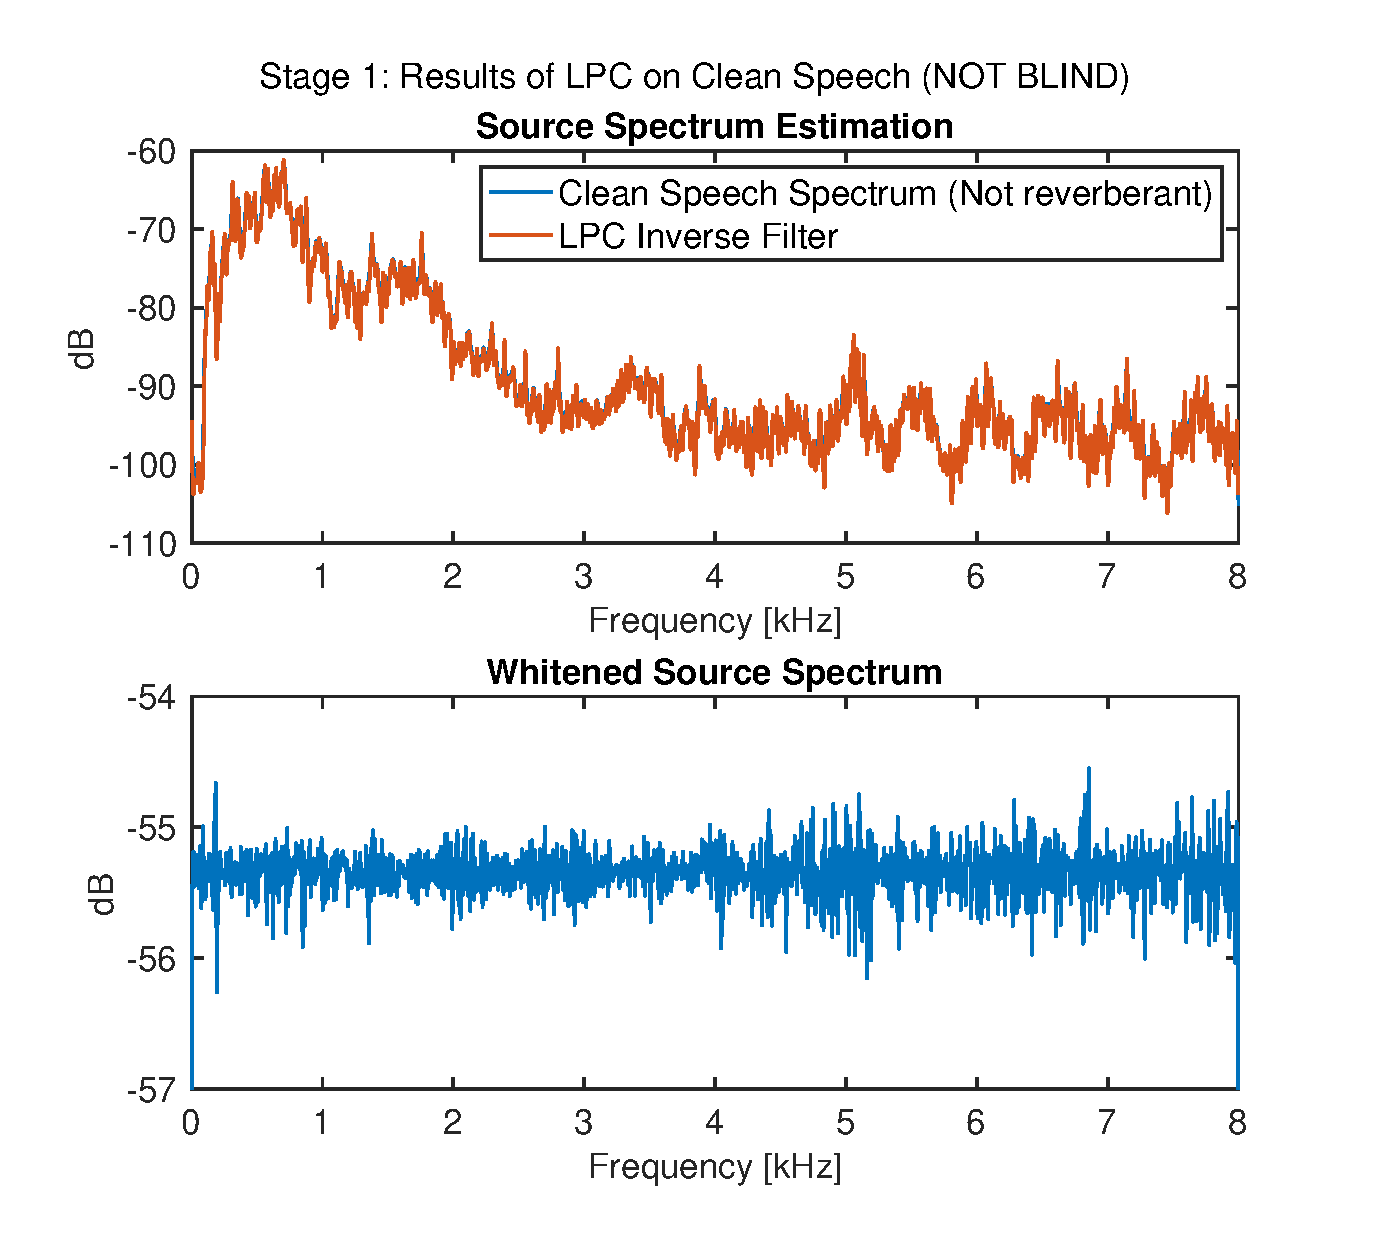
\includegraphics[width=\textwidth]{S1_p1_1000}
	\end{subfigure}
	\hfill
	\begin{subfigure}[b]{0.49\textwidth}
		\centering
		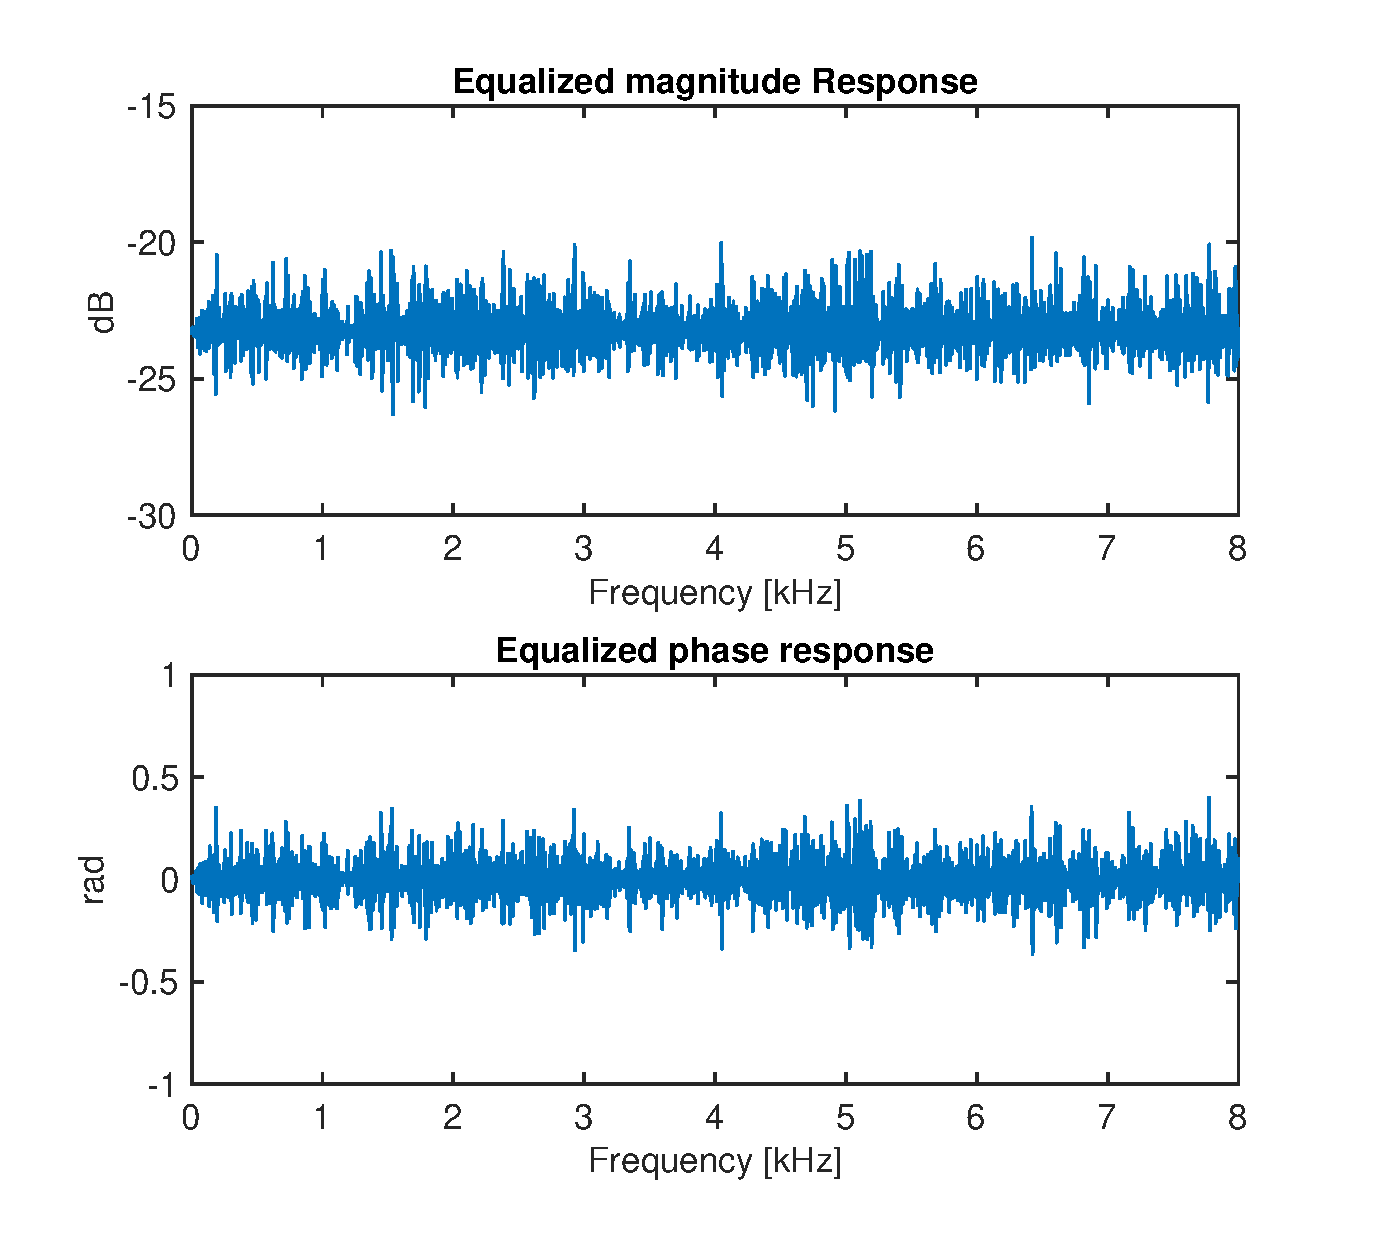
\includegraphics[width=\textwidth]{Equalized_RTF_p1_1000}
	\end{subfigure}
	\hfill
	\begin{subfigure}[b]{0.49\textwidth}
		\centering
		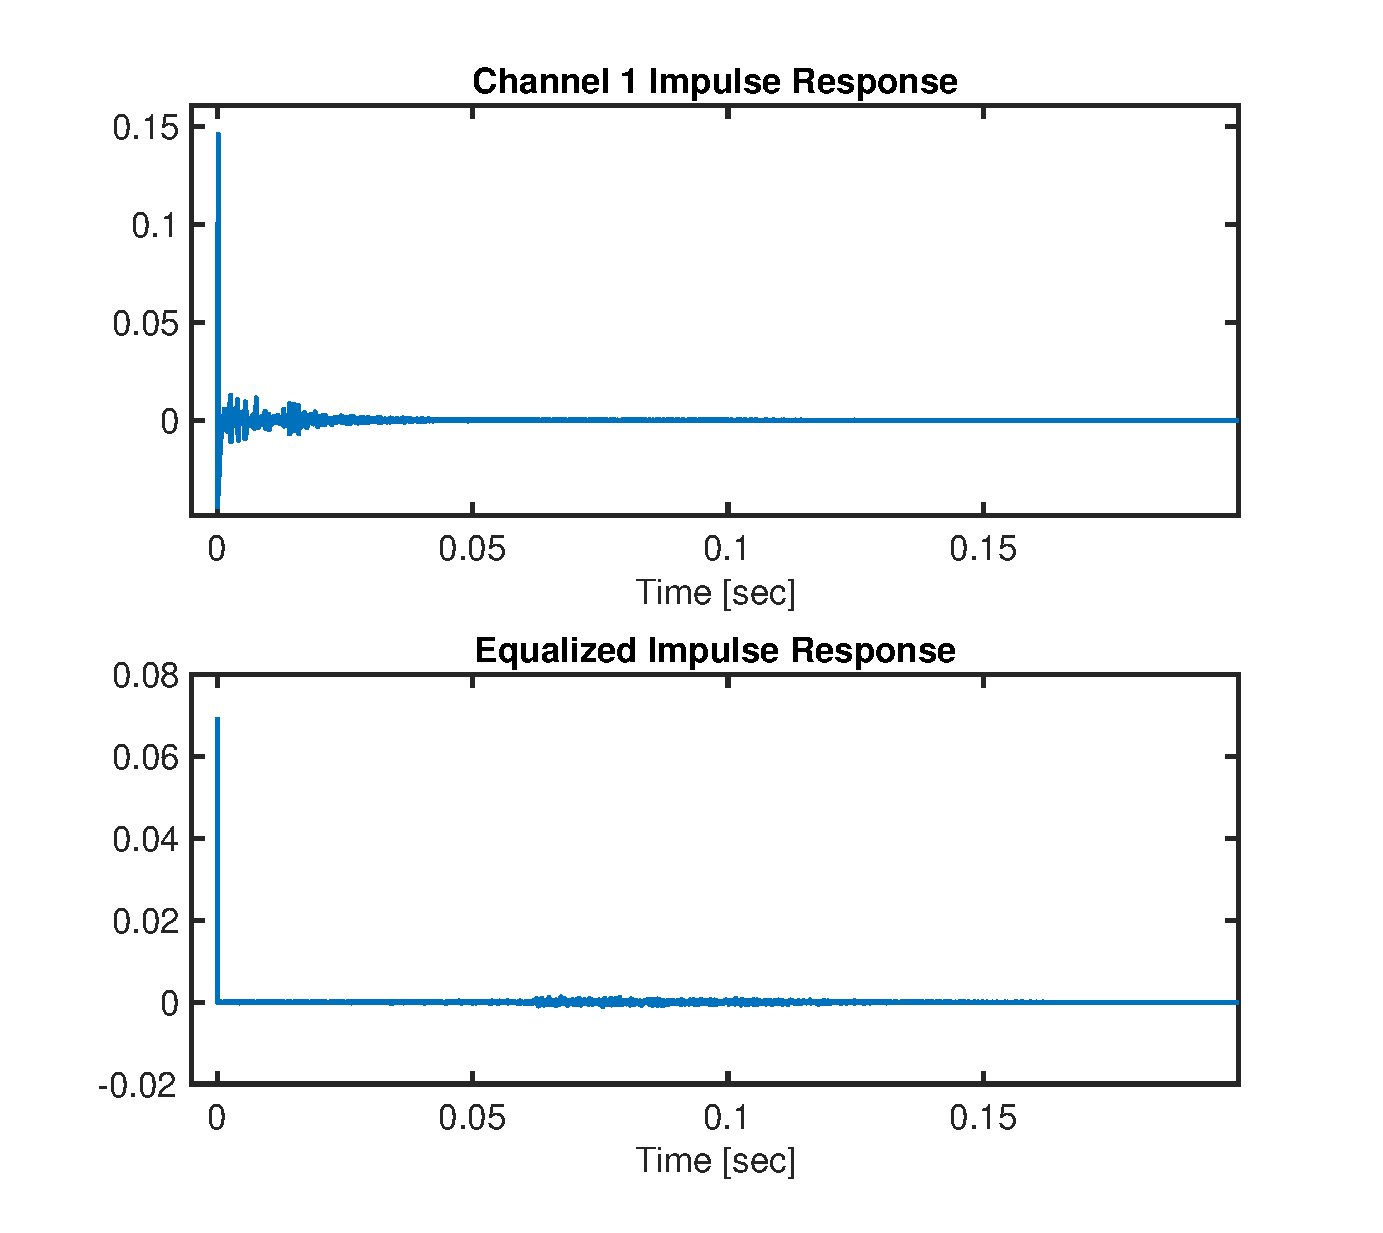
\includegraphics[width=\textwidth]{EIR_p1_1000}
	\end{subfigure}
	\hfill
	\begin{subfigure}[b]{0.49\textwidth}
		\centering
		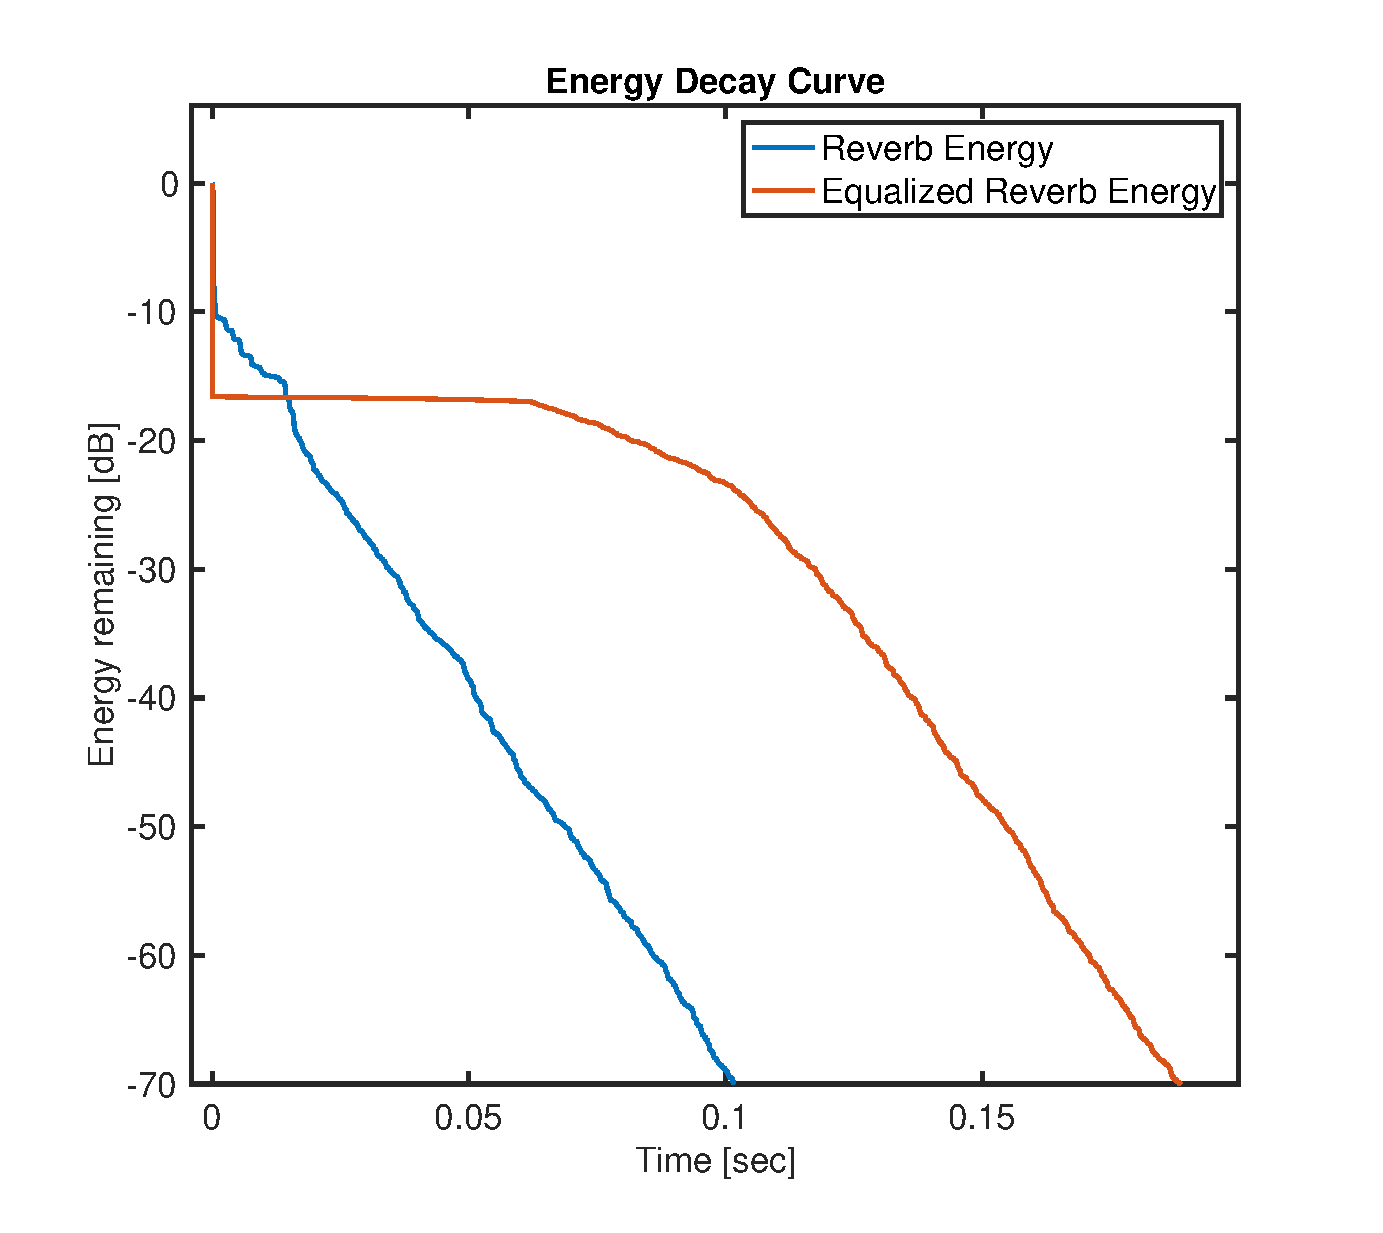
\includegraphics[width=\textwidth]{EDC_p1_1000}
	\end{subfigure}
	\hfill
	\caption[Detailed behaviour of DAP with $p_1 = 1000$]{Delay-and-Predict dereverberation performance with source whitening prediction order $\mathrm{p1} = 1000$ and multichannel linear prediction order $\mathrm{p2} = \mathrm{N60} / (M-1)$.}
	\label{fig:params_p1_1000}
\end{figure}

%\textbf{p1 = p2 * (M-1) (whitened on the same spectral resolution as the MC-LP equalizer)}

\begin{figure}[H]
	\centering
	\begin{subfigure}[b]{0.49\textwidth}
		\centering
		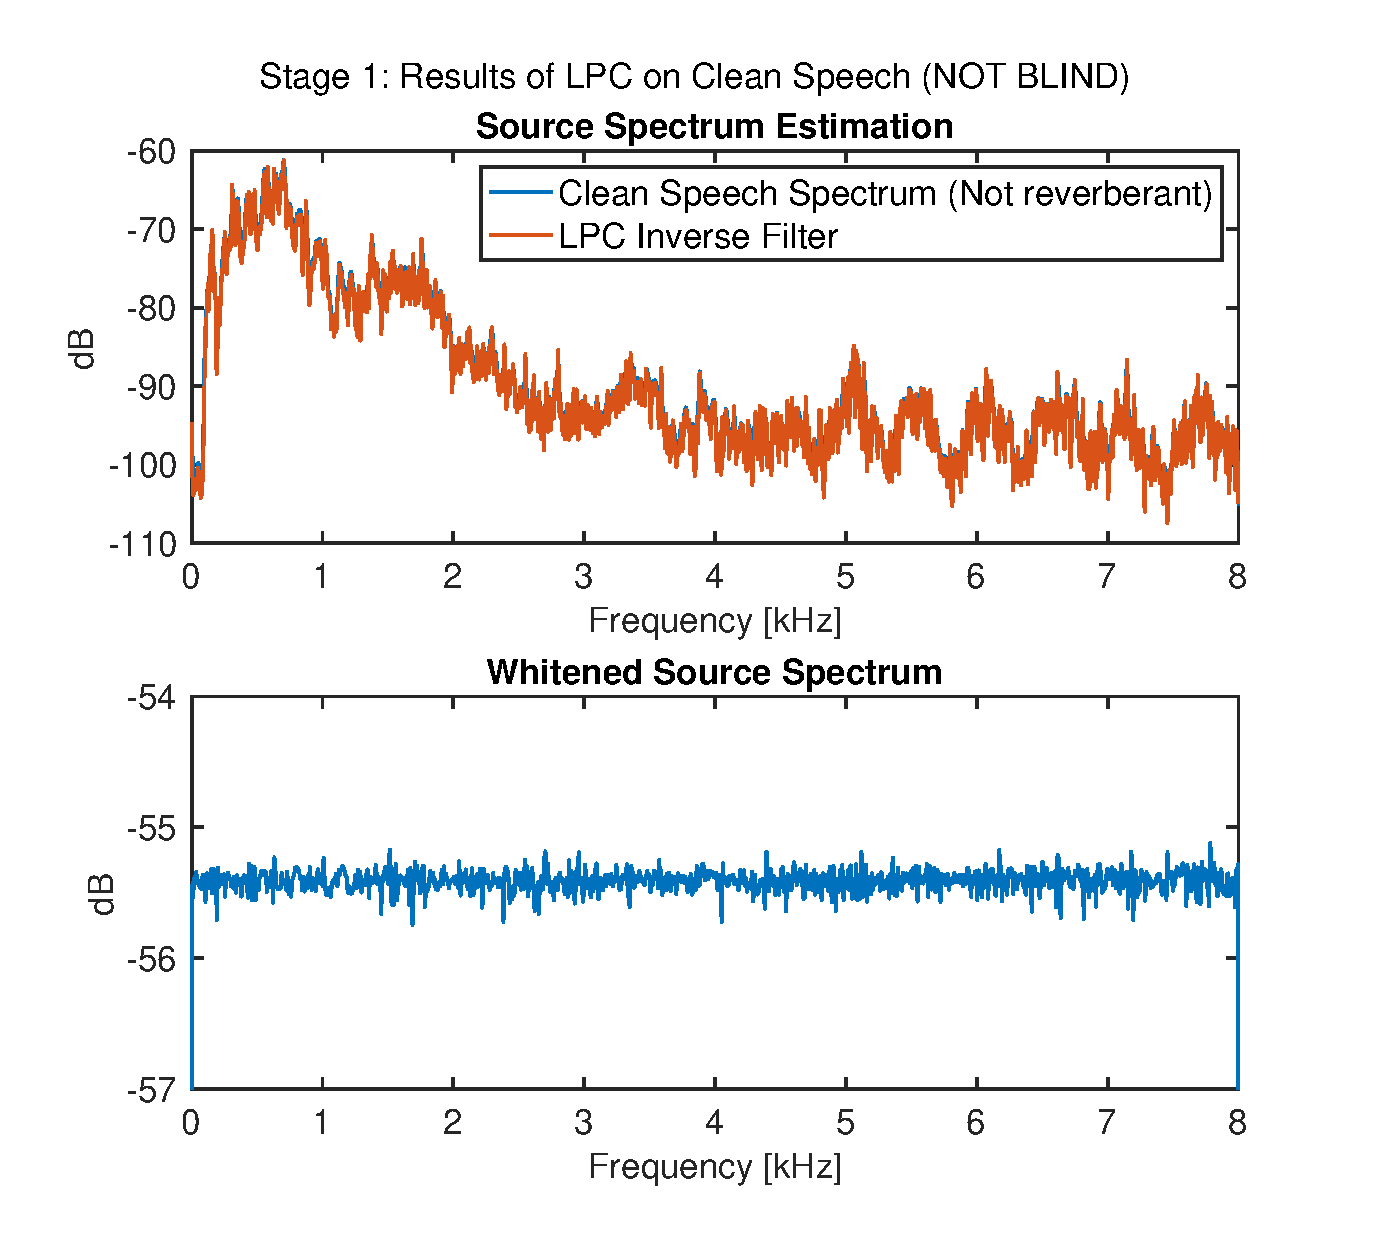
\includegraphics[width=\textwidth]{S1_p1_based_on_p2}
	\end{subfigure}
	\hfill
	\begin{subfigure}[b]{0.49\textwidth}
		\centering
		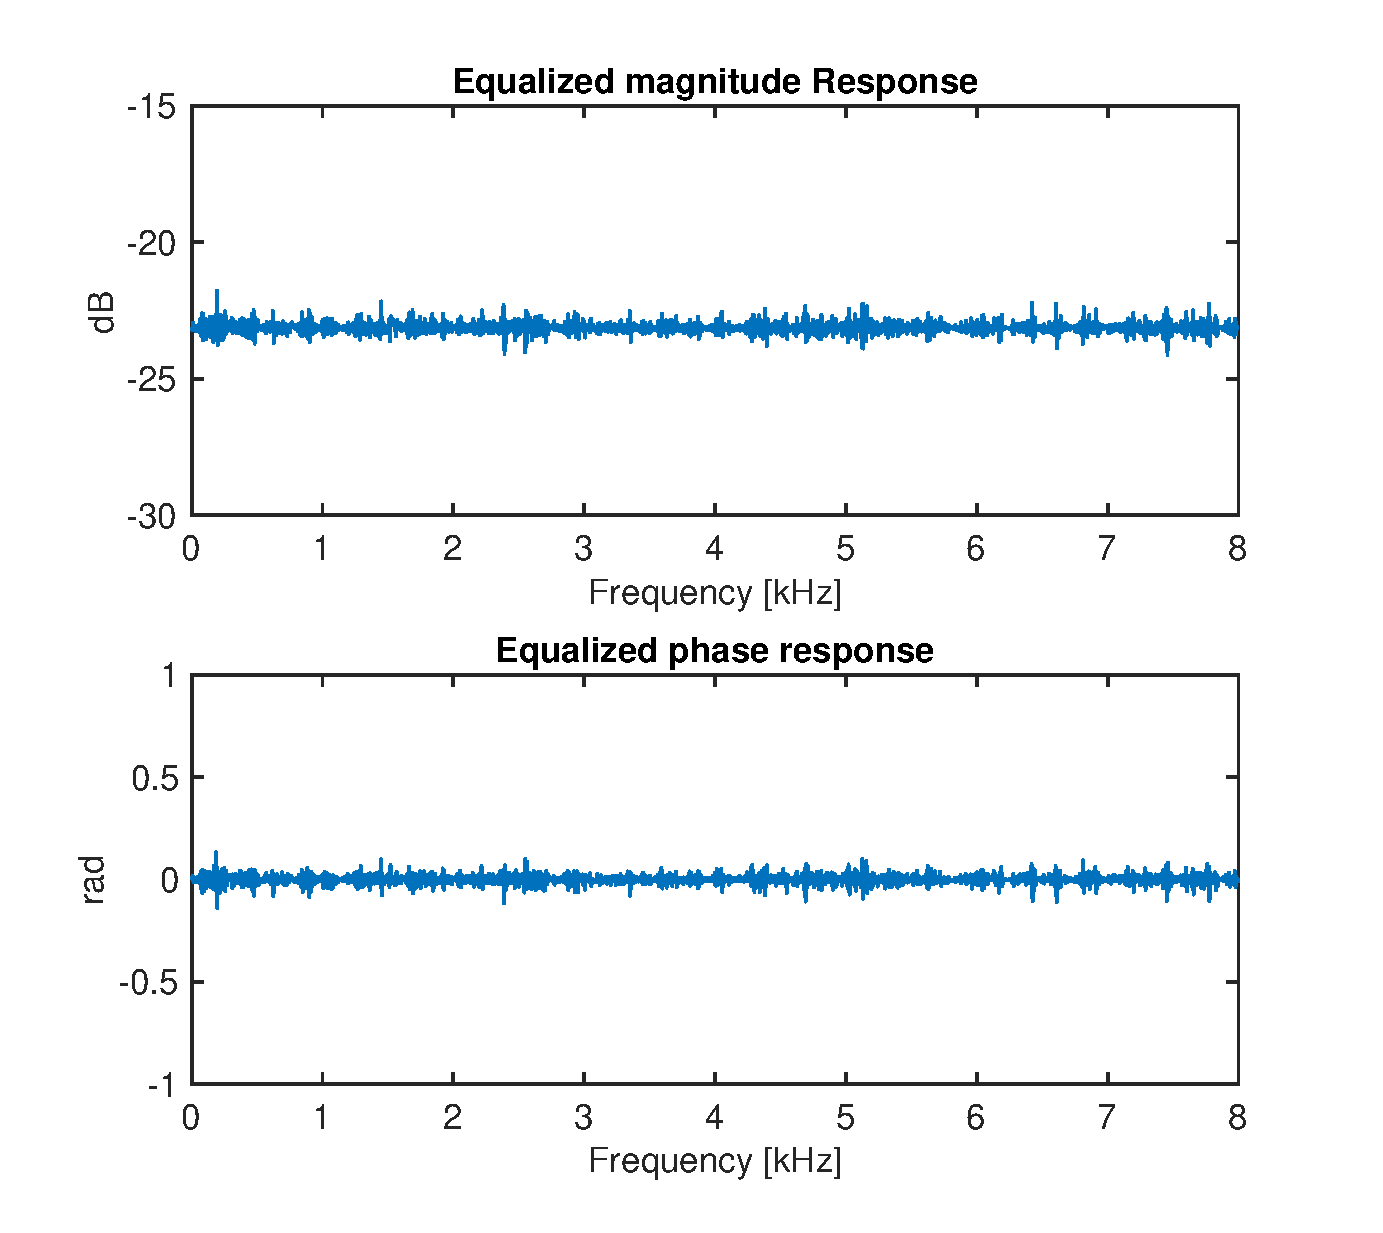
\includegraphics[width=\textwidth]{Equalized_RTF_p1_based_on_p2}
	\end{subfigure}
	\hfill
	\begin{subfigure}[b]{0.49\textwidth}
		\centering
		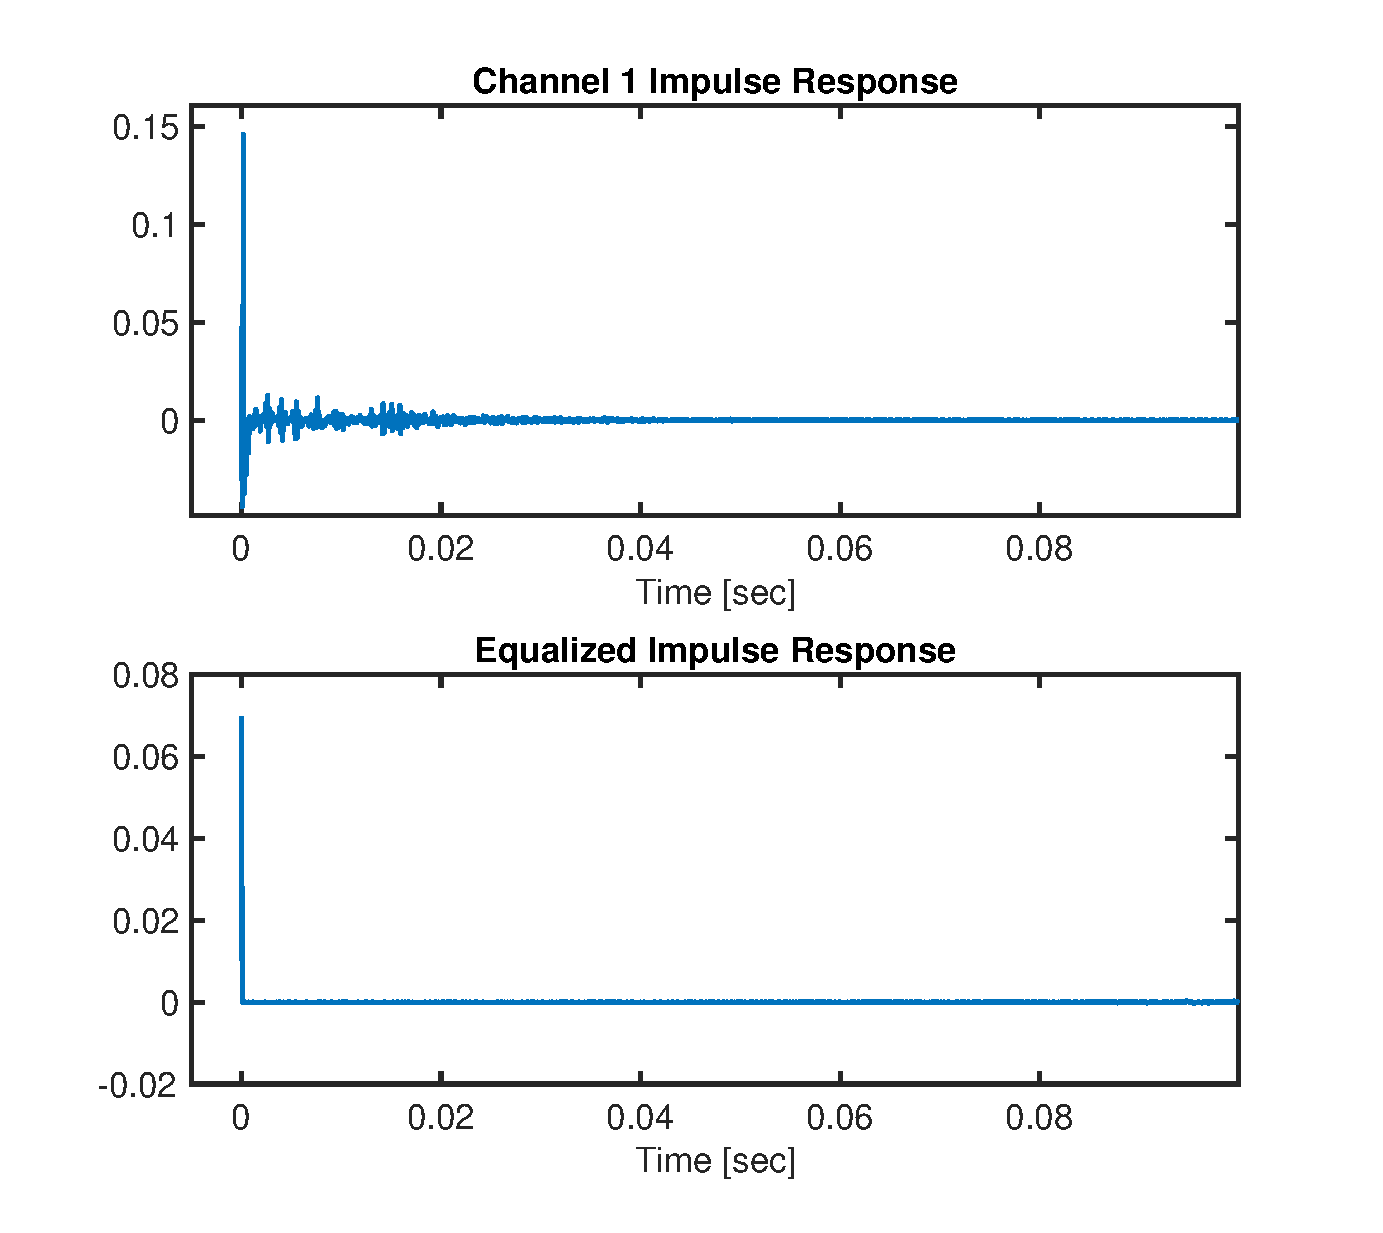
\includegraphics[width=\textwidth]{EIR_p1_based_on_p2}
	\end{subfigure}
	\hfill
	\begin{subfigure}[b]{0.49\textwidth}
		\centering
		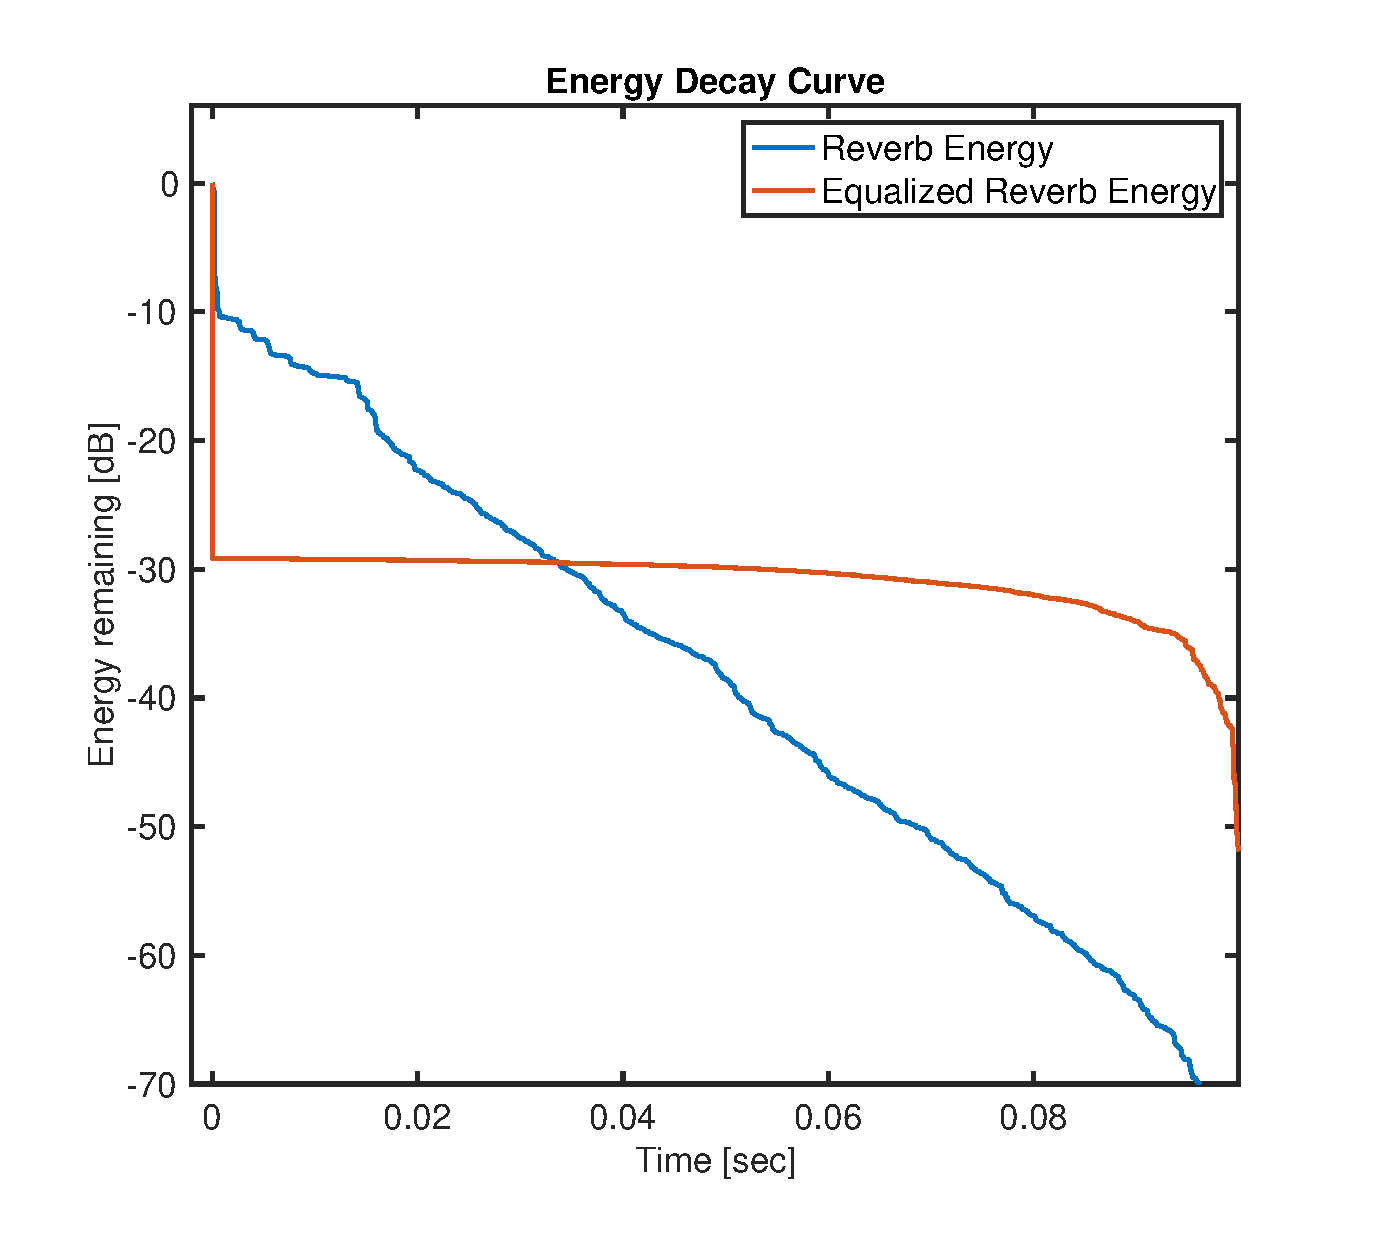
\includegraphics[width=\textwidth]{EDC_p1_based_on_p2}
	\end{subfigure}
	\hfill
	\caption[Detailed behaviour of DAP with $p_1 = p_2 \cdot \left(M-1\right)$]{Delay-and-Predict dereverberation performance with source whitening prediction order $\mathrm{p1} = \mathrm{p2} \cdot (M-1)$ and multichannel linear prediction order $\mathrm{p2} = \mathrm{N60} / (M-1)$. I.e., The source whitening filter order is the same as the effective MINT filter order.}
	\label{fig:params_p1_based_on_p2}
\end{figure}

%\textbf{p1 = 2 * p2  * (M-1) (Extra headroom)}

\begin{figure}[H]
	\centering
	\begin{subfigure}[b]{0.49\textwidth}
		\centering
		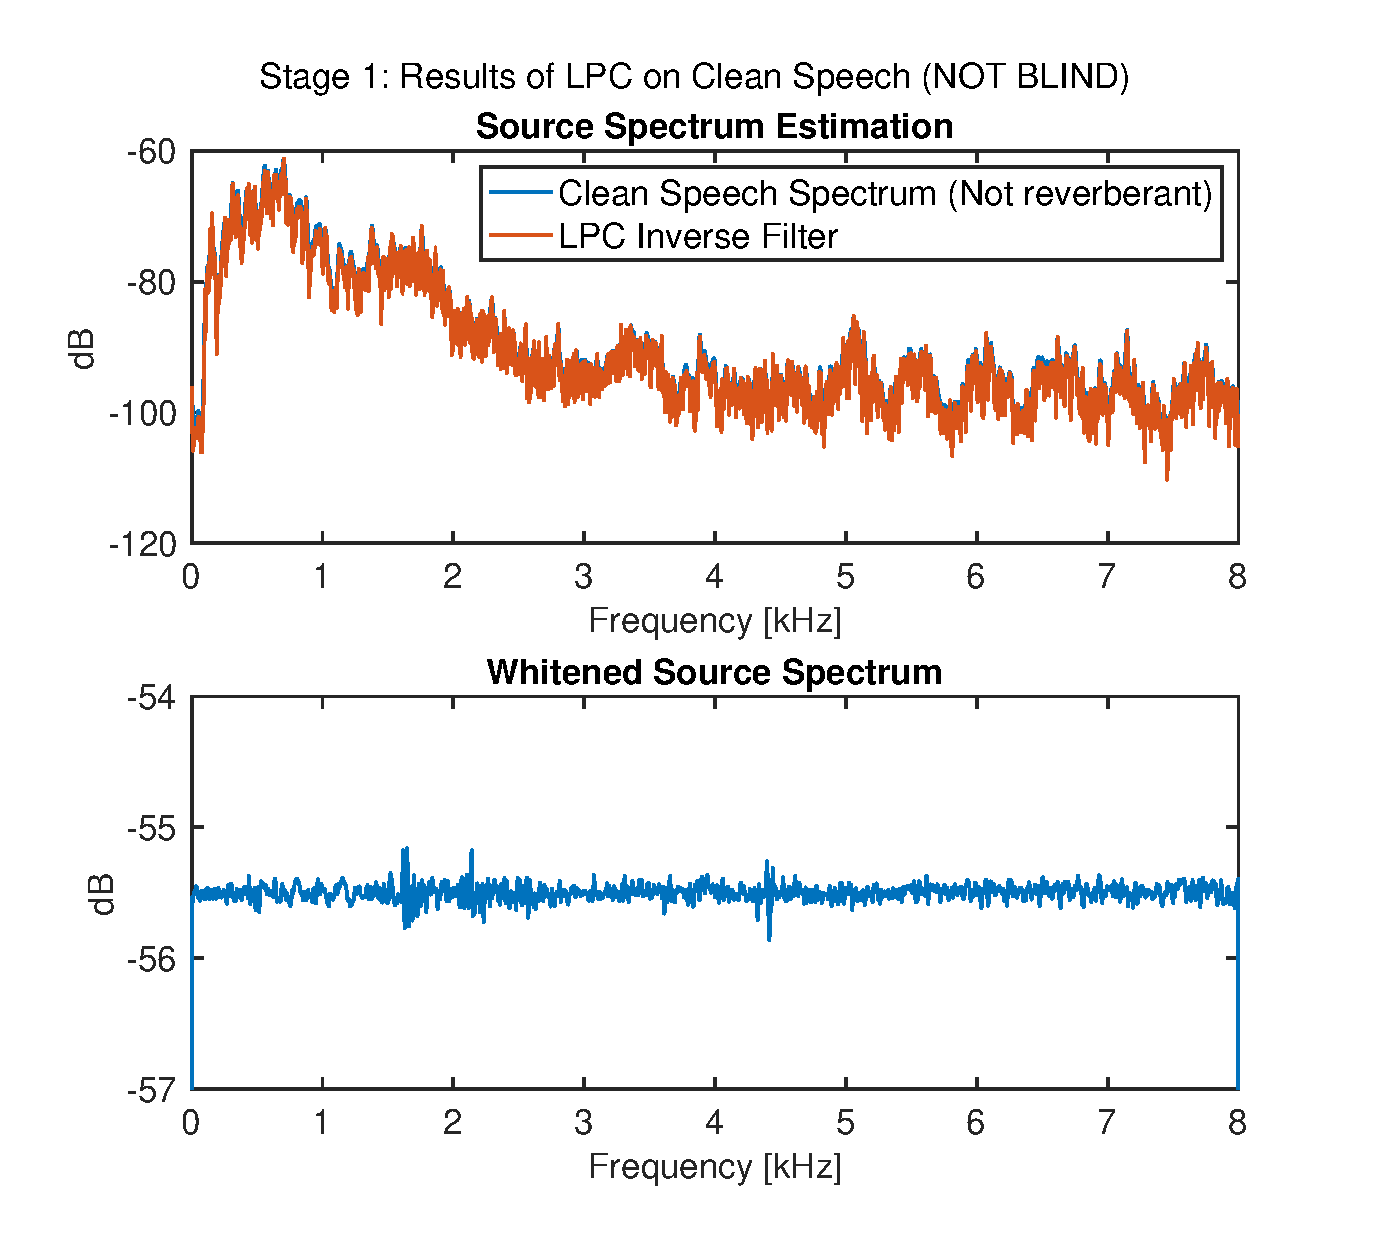
\includegraphics[width=\textwidth]{S1_p1_2x_p2}
	\end{subfigure}
	\hfill
	\begin{subfigure}[b]{0.49\textwidth}
		\centering
		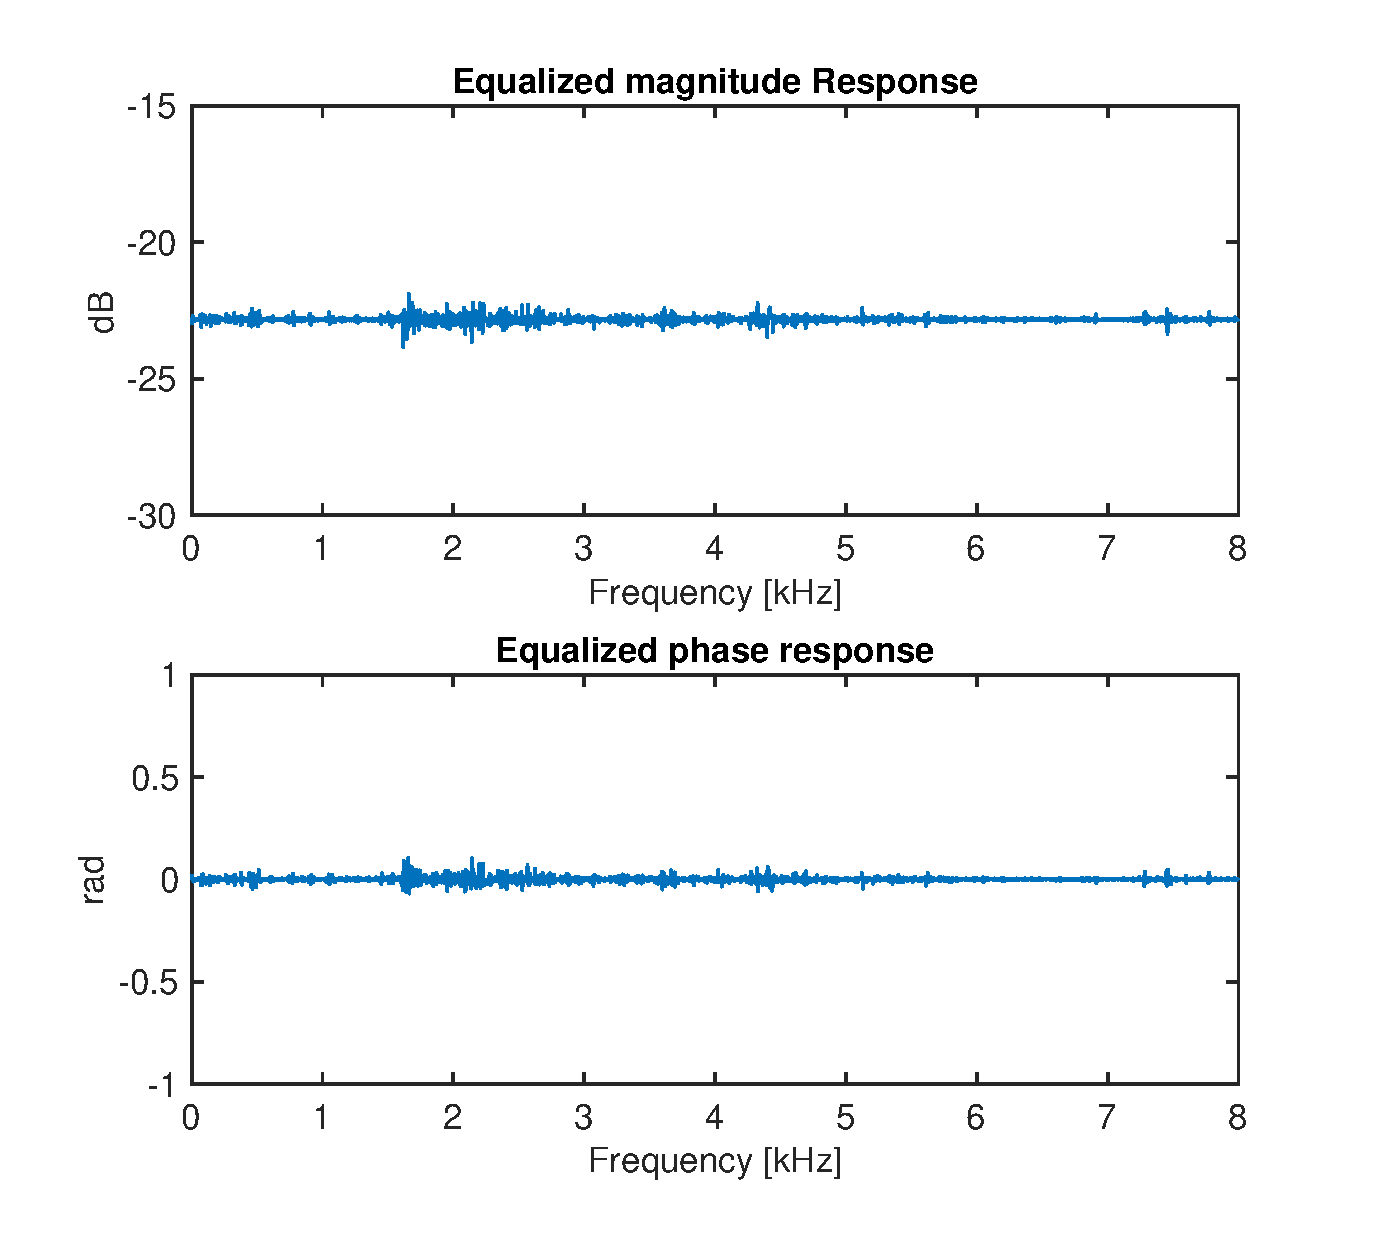
\includegraphics[width=\textwidth]{Equalized_RTF_p1_2x_p2}
	\end{subfigure}
	\hfill
	\begin{subfigure}[b]{0.49\textwidth}
		\centering
		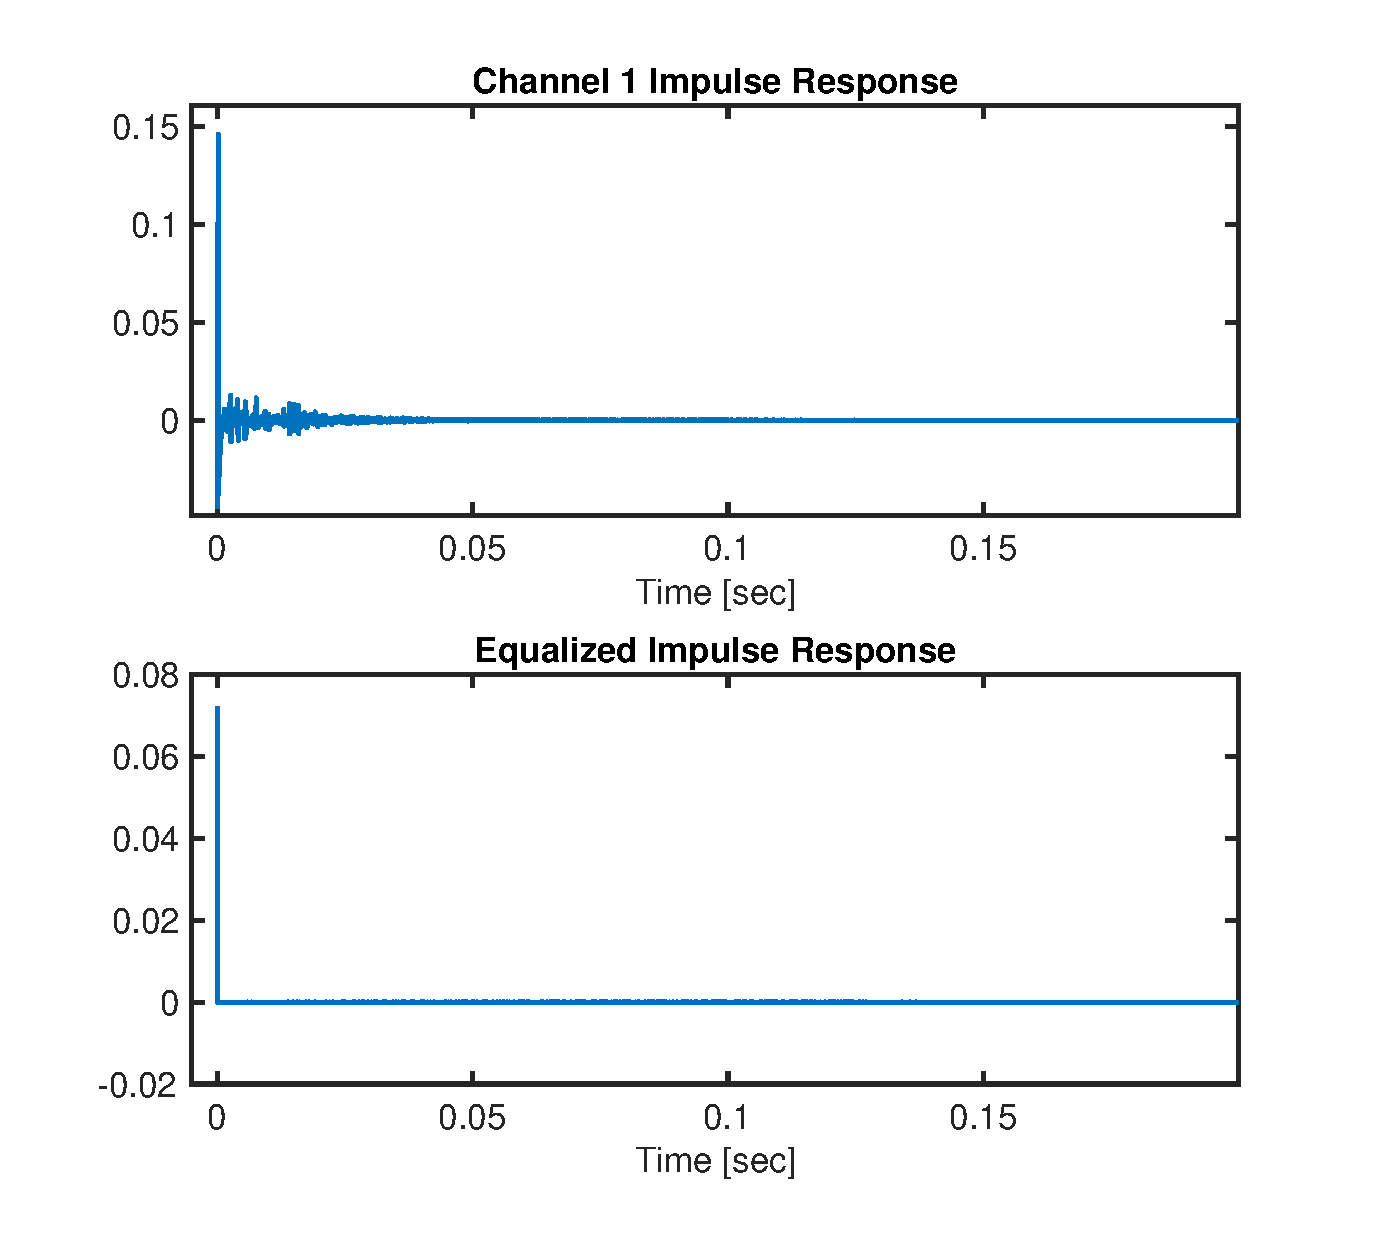
\includegraphics[width=\textwidth]{EIR_p1_2x_p2}
	\end{subfigure}
	\hfill
	\begin{subfigure}[b]{0.49\textwidth}
		\centering
		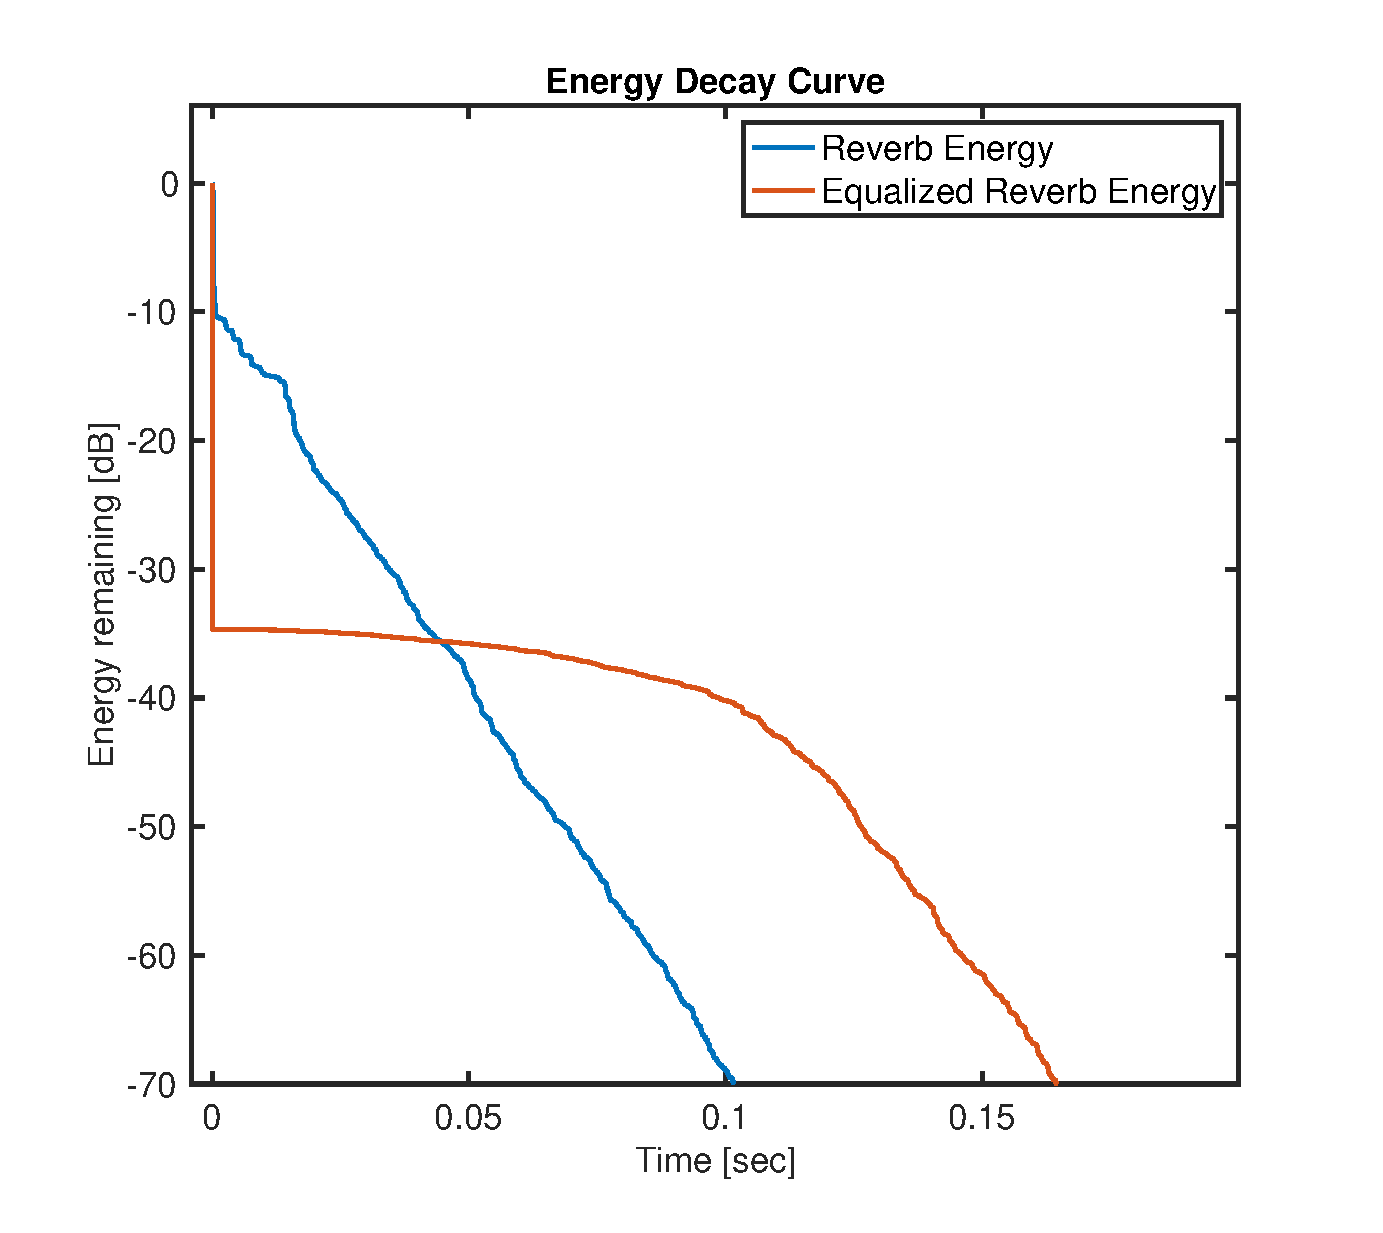
\includegraphics[width=\textwidth]{EDC_p1_2x_p2}
	\end{subfigure}
	\hfill
	\caption[Detailed behaviour of DAP with $p_1 = 2 \cdot p_2 \cdot \left(M-1\right)$]{Delay-and-Predict dereverberation performance with source whitening prediction order $\mathrm{p1} = 2 \cdot \mathrm{p2} \cdot (M-1)$ and multichannel linear prediction order $\mathrm{p2} = \mathrm{N60} / (M-1)$. I.e., The source whitening filter order is twice the effective MINT filter order.}
	\label{fig:params_p1_2x_p2}
\end{figure}

%... beyond about p1 = 1.25 * p2 * (M-1) EDC performance saturates at approximately -35 dB reverb attenuation.


\section{Chapter 4 Additional Figures}

\subsection{EC Evaluation} \label{section:appendix:EC_eval}


\begin{figure}[H]
	\centering
	\begin{subfigure}[b]{0.49\textwidth}
		\centering
		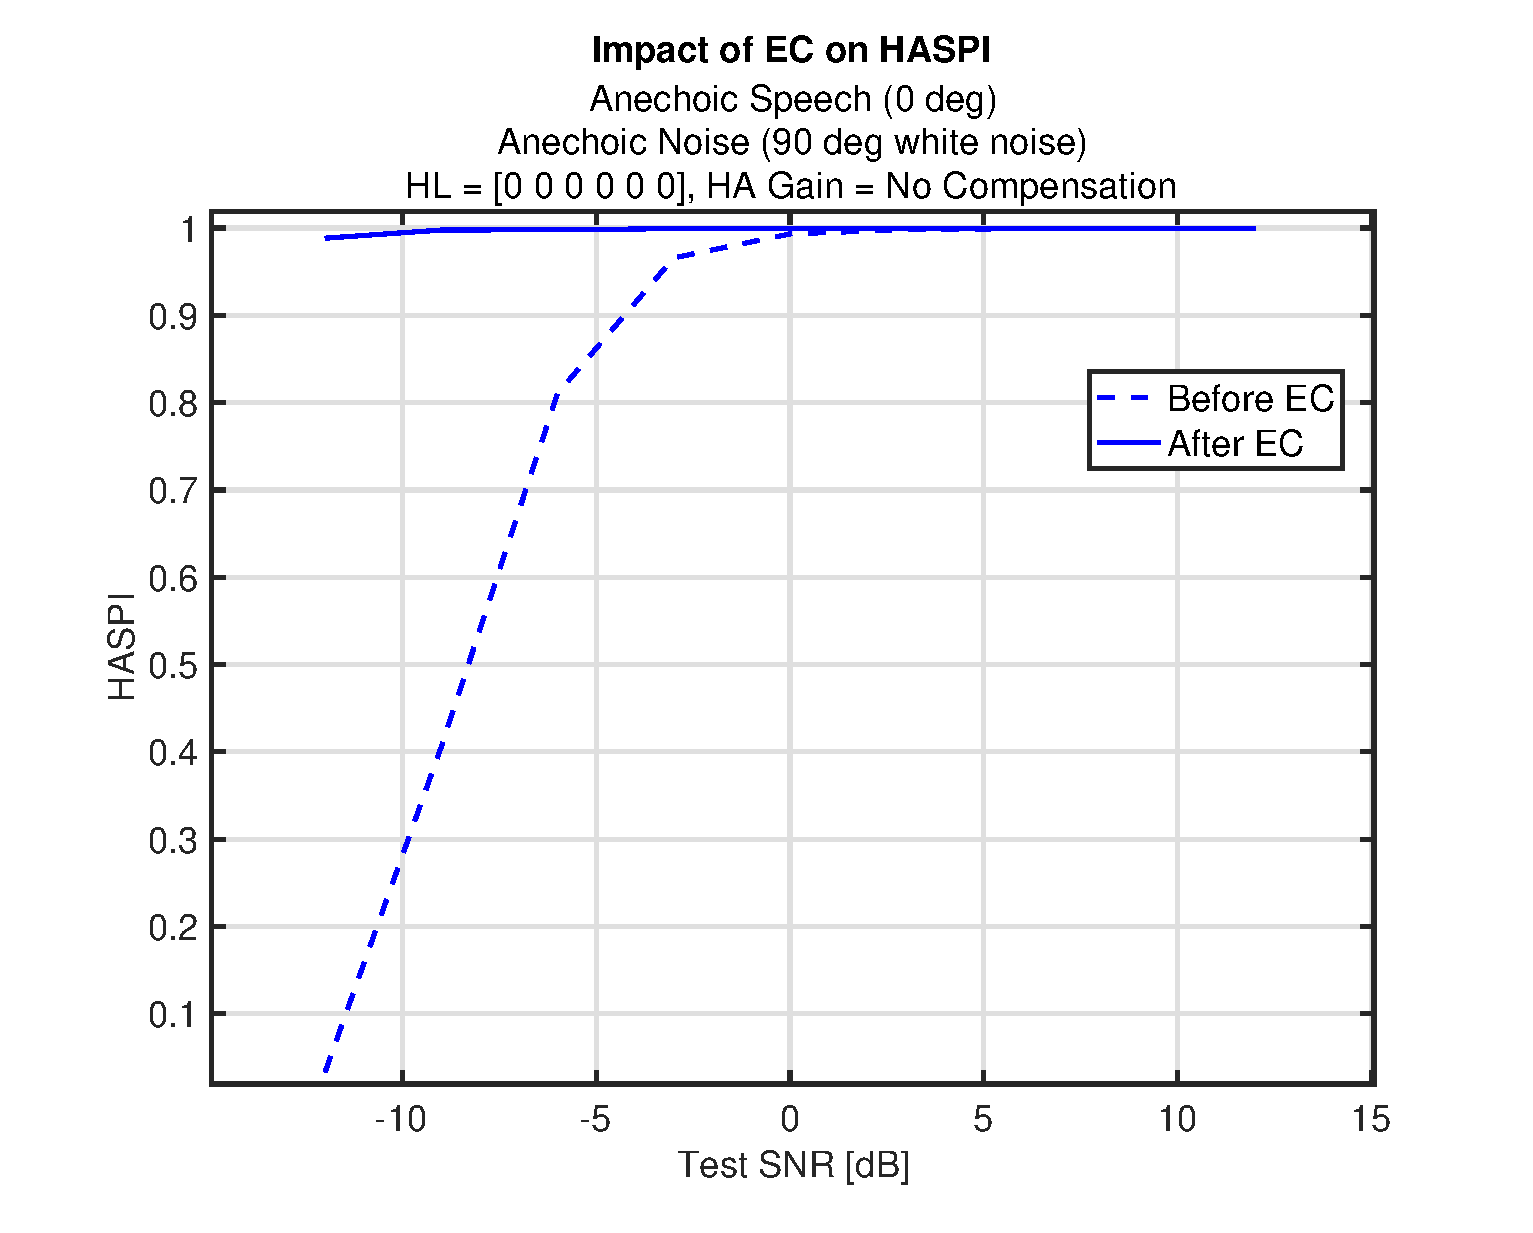
\includegraphics[width=\textwidth]{EC_SRM_AnechoicSpeech_AnechoicNoise}
	\end{subfigure}
	\hfill
	\begin{subfigure}[b]{0.49\textwidth}
		\centering
		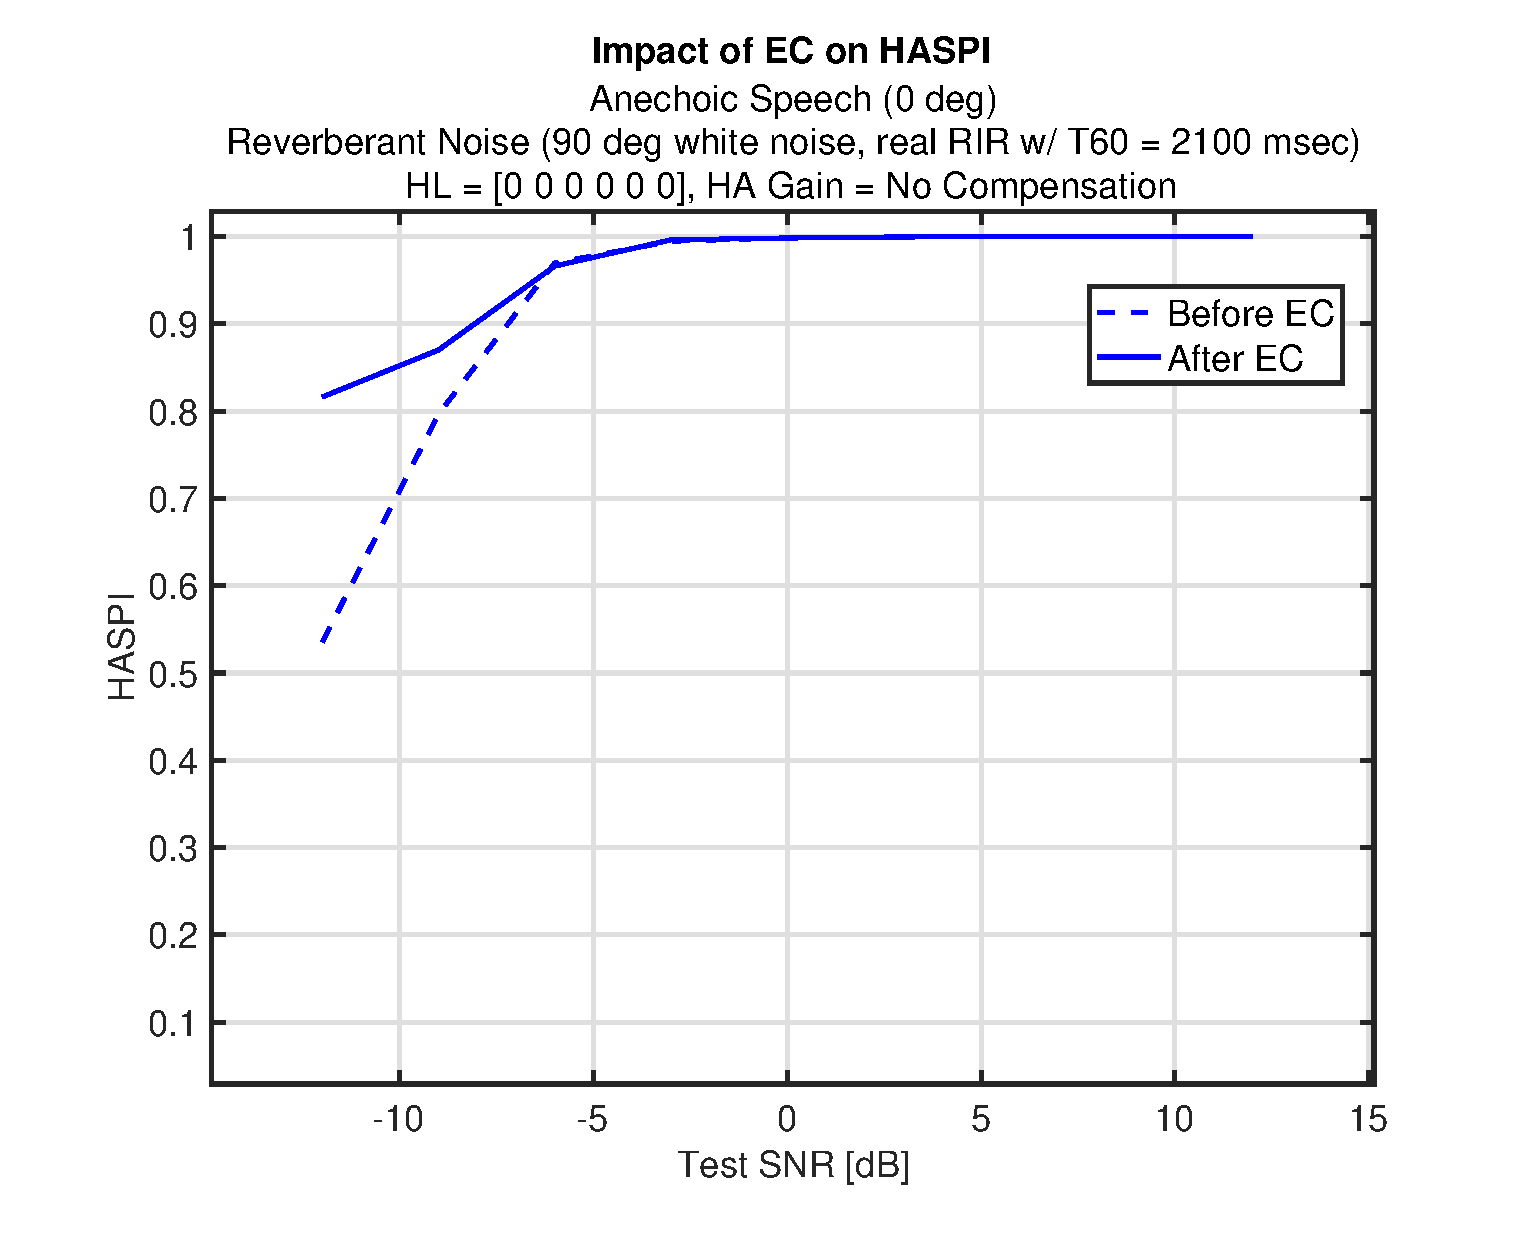
\includegraphics[width=\textwidth]{EC_SRM_AnechoicSpeech_ReverbNoise}
	\end{subfigure}
	\hfill
	\begin{subfigure}[b]{0.49\textwidth}
		\centering
		\includegraphics[width=\textwidth]{EC_SRM_AnechoicSpeech_SpatialNoiseRecording}
	\end{subfigure}
	\hfill
	\begin{subfigure}[b]{0.49\textwidth}
		\centering
		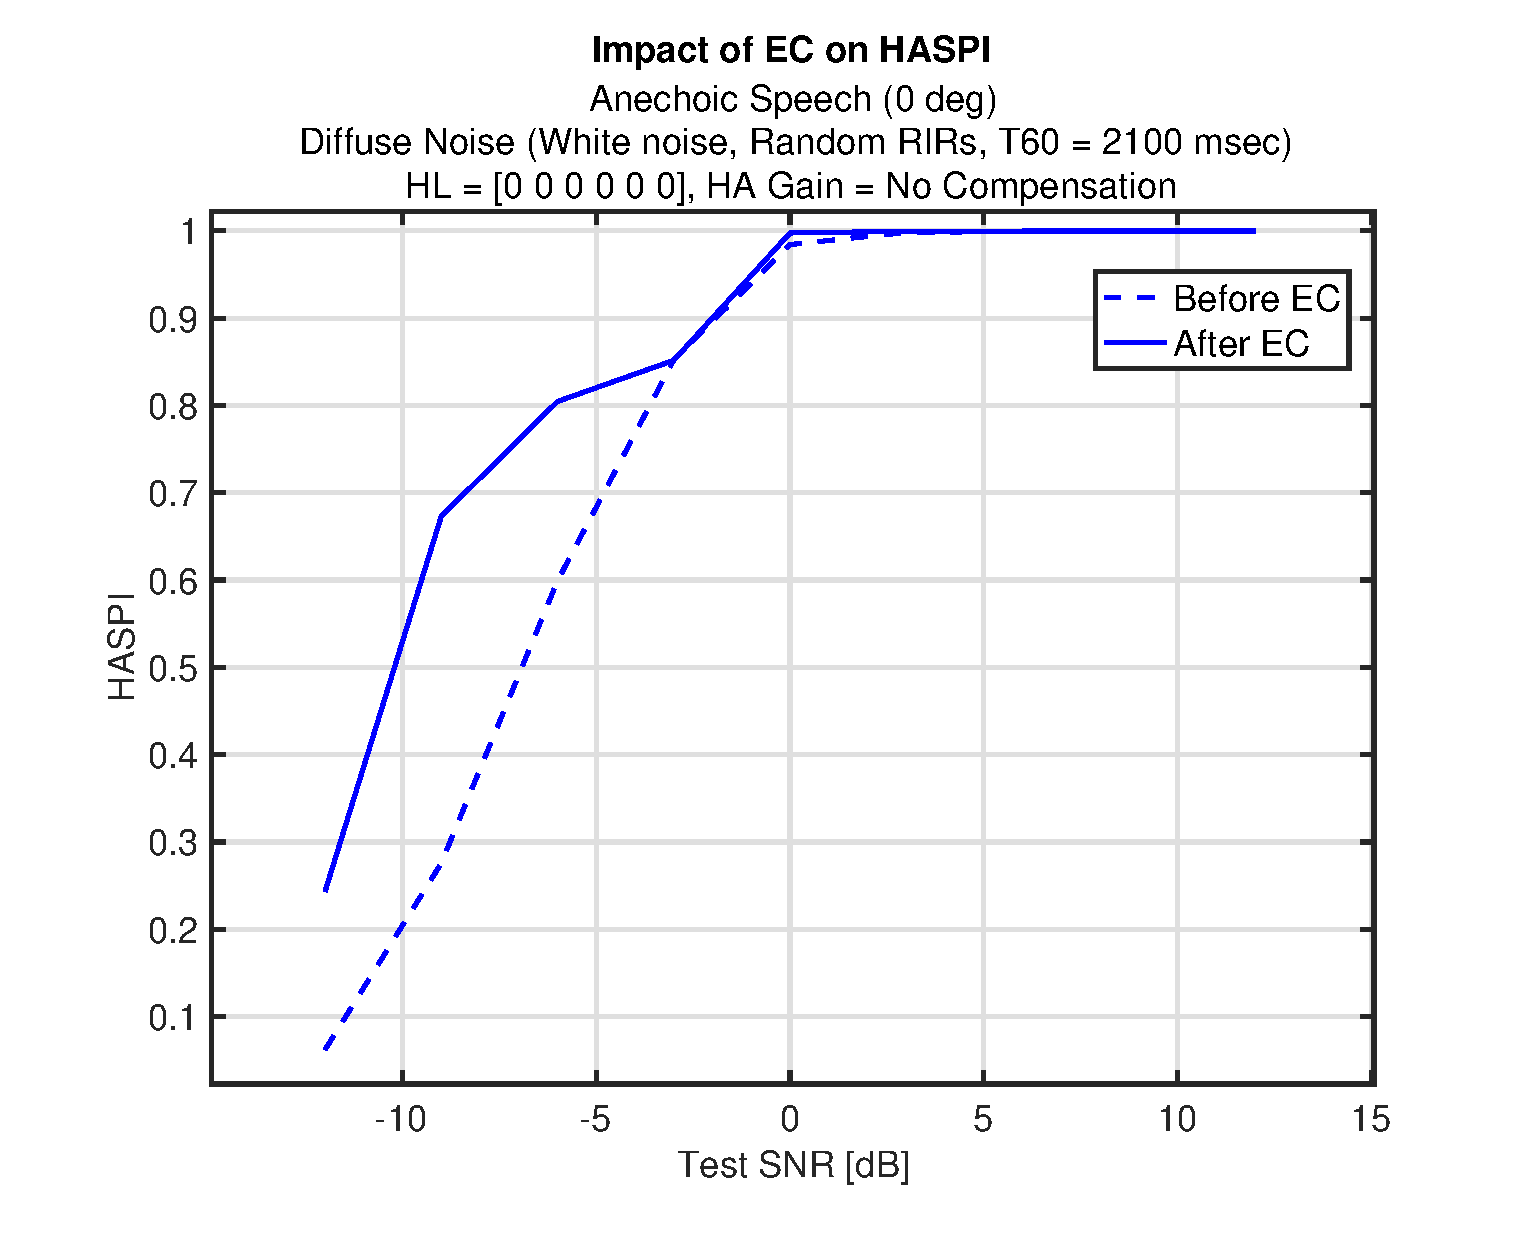
\includegraphics[width=\textwidth]{EC_SRM_AnechoicSpeech_DiffuseNoise}
	\end{subfigure}
	\hfill
	\caption[EC front-end performance with anechoic speech]{Impact of EC algorithm on speech intelligibility (using HASPI) as a function of SNR, for anechoic directional speech and various noise types (anechoic directional, reverberant, spatial recording, diffuse)}
	\label{fig:EC_SRM_AnechoicSpeech}
\end{figure}


\begin{figure}[H]
	\centering
	\begin{subfigure}[b]{0.49\textwidth}
		\centering
		\includegraphics[width=\textwidth]{EC_SRM_ReverbSpeech_AnechoicNoise}
	\end{subfigure}
	\hfill
	\begin{subfigure}[b]{0.49\textwidth}
		\centering
		\includegraphics[width=\textwidth]{EC_SRM_ReverbSpeech_ReverbNoise}
	\end{subfigure}
	\hfill
	\begin{subfigure}[b]{0.49\textwidth}
		\centering
		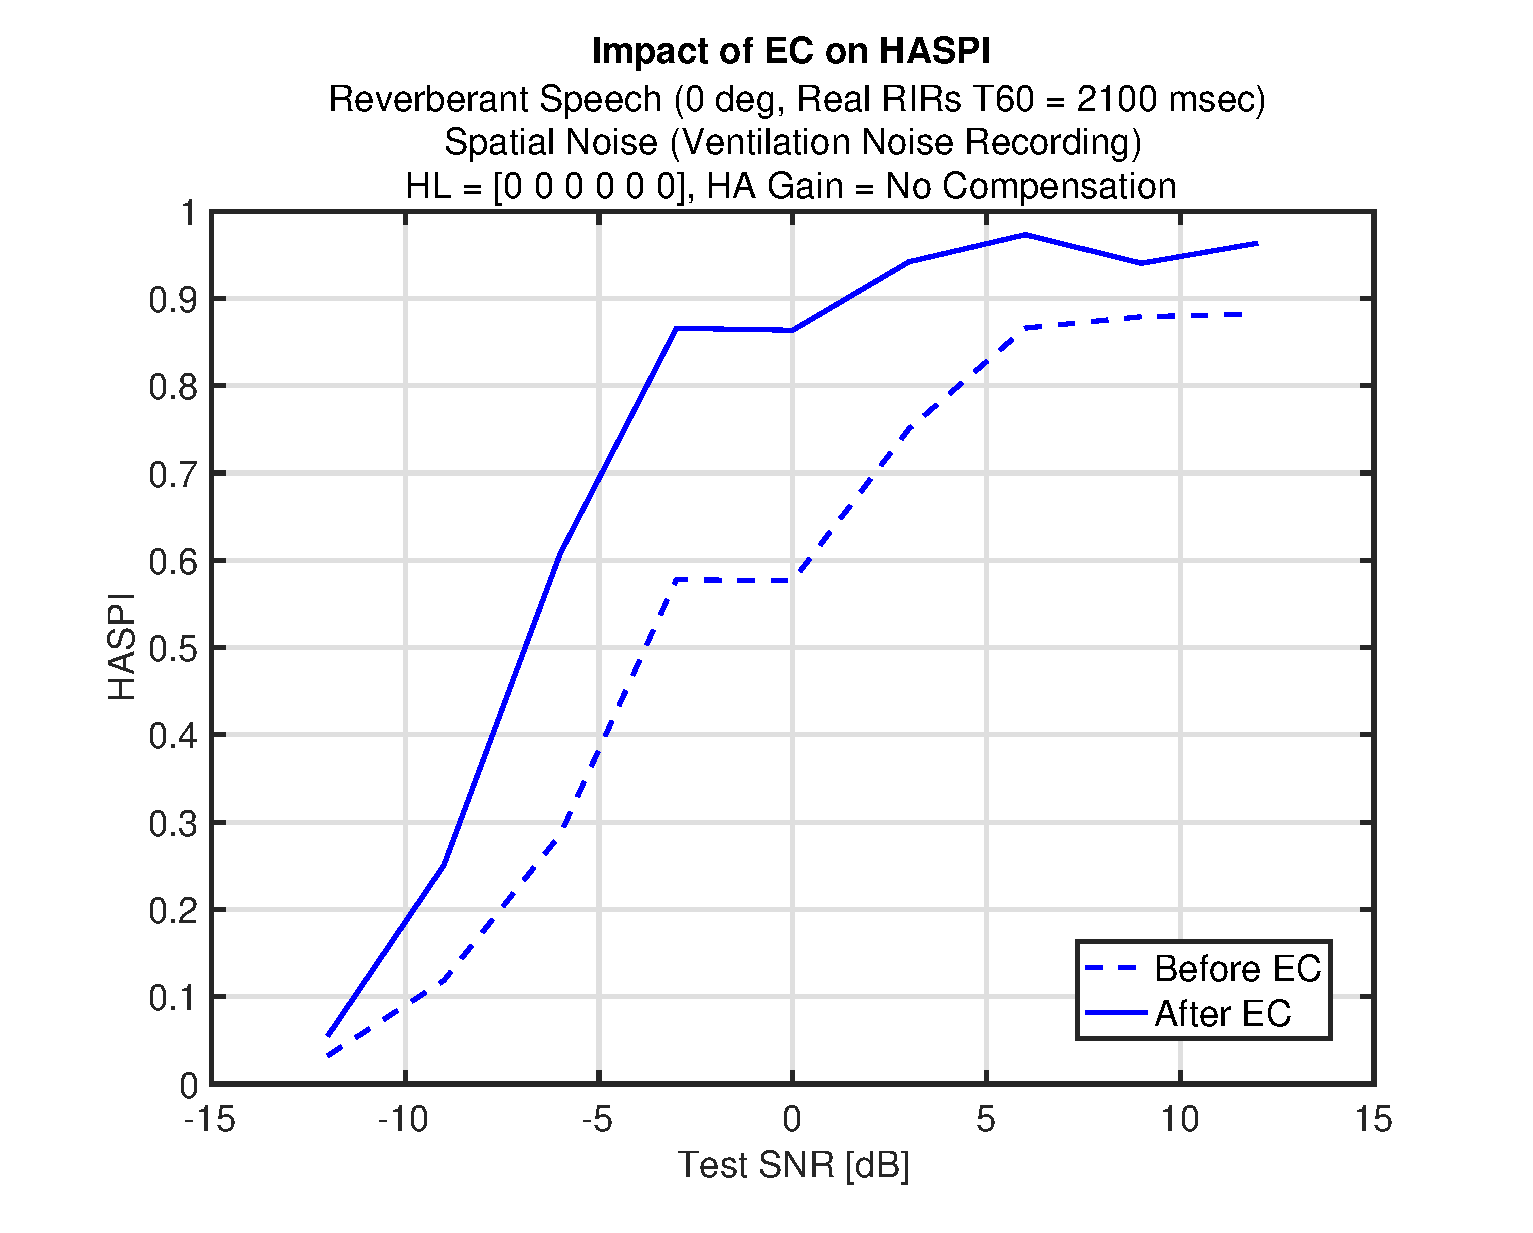
\includegraphics[width=\textwidth]{EC_SRM_ReverbSpeech_SpatialNoiseRecording}
	\end{subfigure}
	\hfill
	\begin{subfigure}[b]{0.49\textwidth}
		\centering
		\includegraphics[width=\textwidth]{EC_SRM_ReverbSpeech_DiffuseNoise}
	\end{subfigure}
	\hfill
	\caption[EC front-end performance with reverberant speech]{Impact of EC algorithm on speech intelligibility (using HASPI) as a function of SNR, for reverberant speech and various noise types (anechoic directional, reverberant, spatial recording, diffuse)}
	\label{fig:EC_SRM_ReverbSpeech}
\end{figure}


\begin{figure}[H]
	\centering
	\begin{subfigure}[b]{0.49\textwidth}
		\centering
		\includegraphics[width=\textwidth]{EC_SRM_DiffuseSpeech_AnechoicNoise}
	\end{subfigure}
	\hfill
	\begin{subfigure}[b]{0.49\textwidth}
		\centering
		\includegraphics[width=\textwidth]{EC_SRM_DiffuseSpeech_ReverbNoise}
	\end{subfigure}
	\hfill
	\begin{subfigure}[b]{0.49\textwidth}
		\centering
		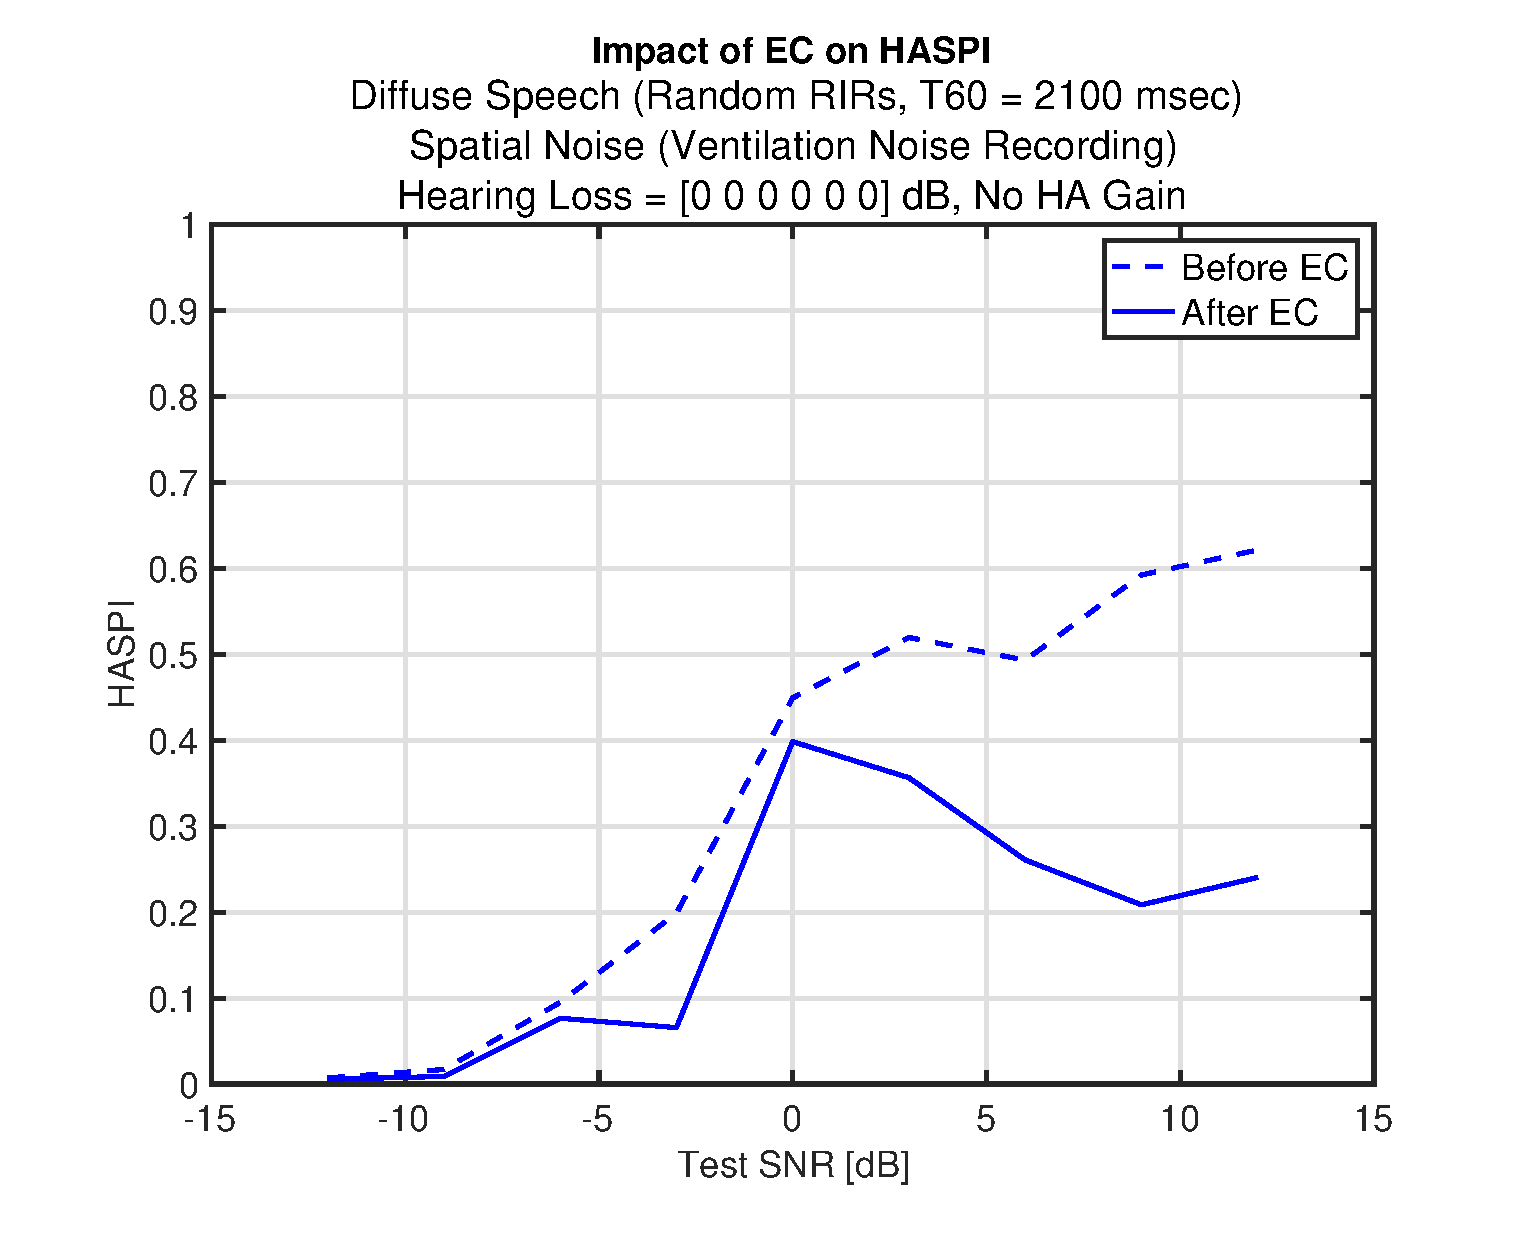
\includegraphics[width=\textwidth]{EC_SRM_DiffuseSpeech_SpatialNoiseRecording}
	\end{subfigure}
	\hfill
	\begin{subfigure}[b]{0.49\textwidth}
		\centering
		\includegraphics[width=\textwidth]{EC_SRM_DiffuseSpeech_DiffuseNoise}
	\end{subfigure}
	\hfill
	\caption[EC front-end performance with diffuse speech]{Impact of EC algorithm on speech intelligibility (using HASPI) as a function of SNR, for diffuse speech and various noise types (anechoic directional, reverberant, spatial recording, diffuse)}
	\label{fig:EC_SRM_DiffuseSpeech}
\end{figure}

\subsection{Higher Order Delay-and-Predict Dereverberation Evaluation in Variable Reverberation with regularization} \label{section:appendix:DAP_EVAL_1000p2wReg}

\begin{figure}[H]
	\centering
	\begin{subfigure}[b]{0.47\textwidth}
		\centering
		\includegraphics[width=\textwidth]{DAP_EVAL_1000T60max_wReg_C50_v_T60}
	\end{subfigure}
	\begin{subfigure}[b]{0.92\textwidth}
		\centering
		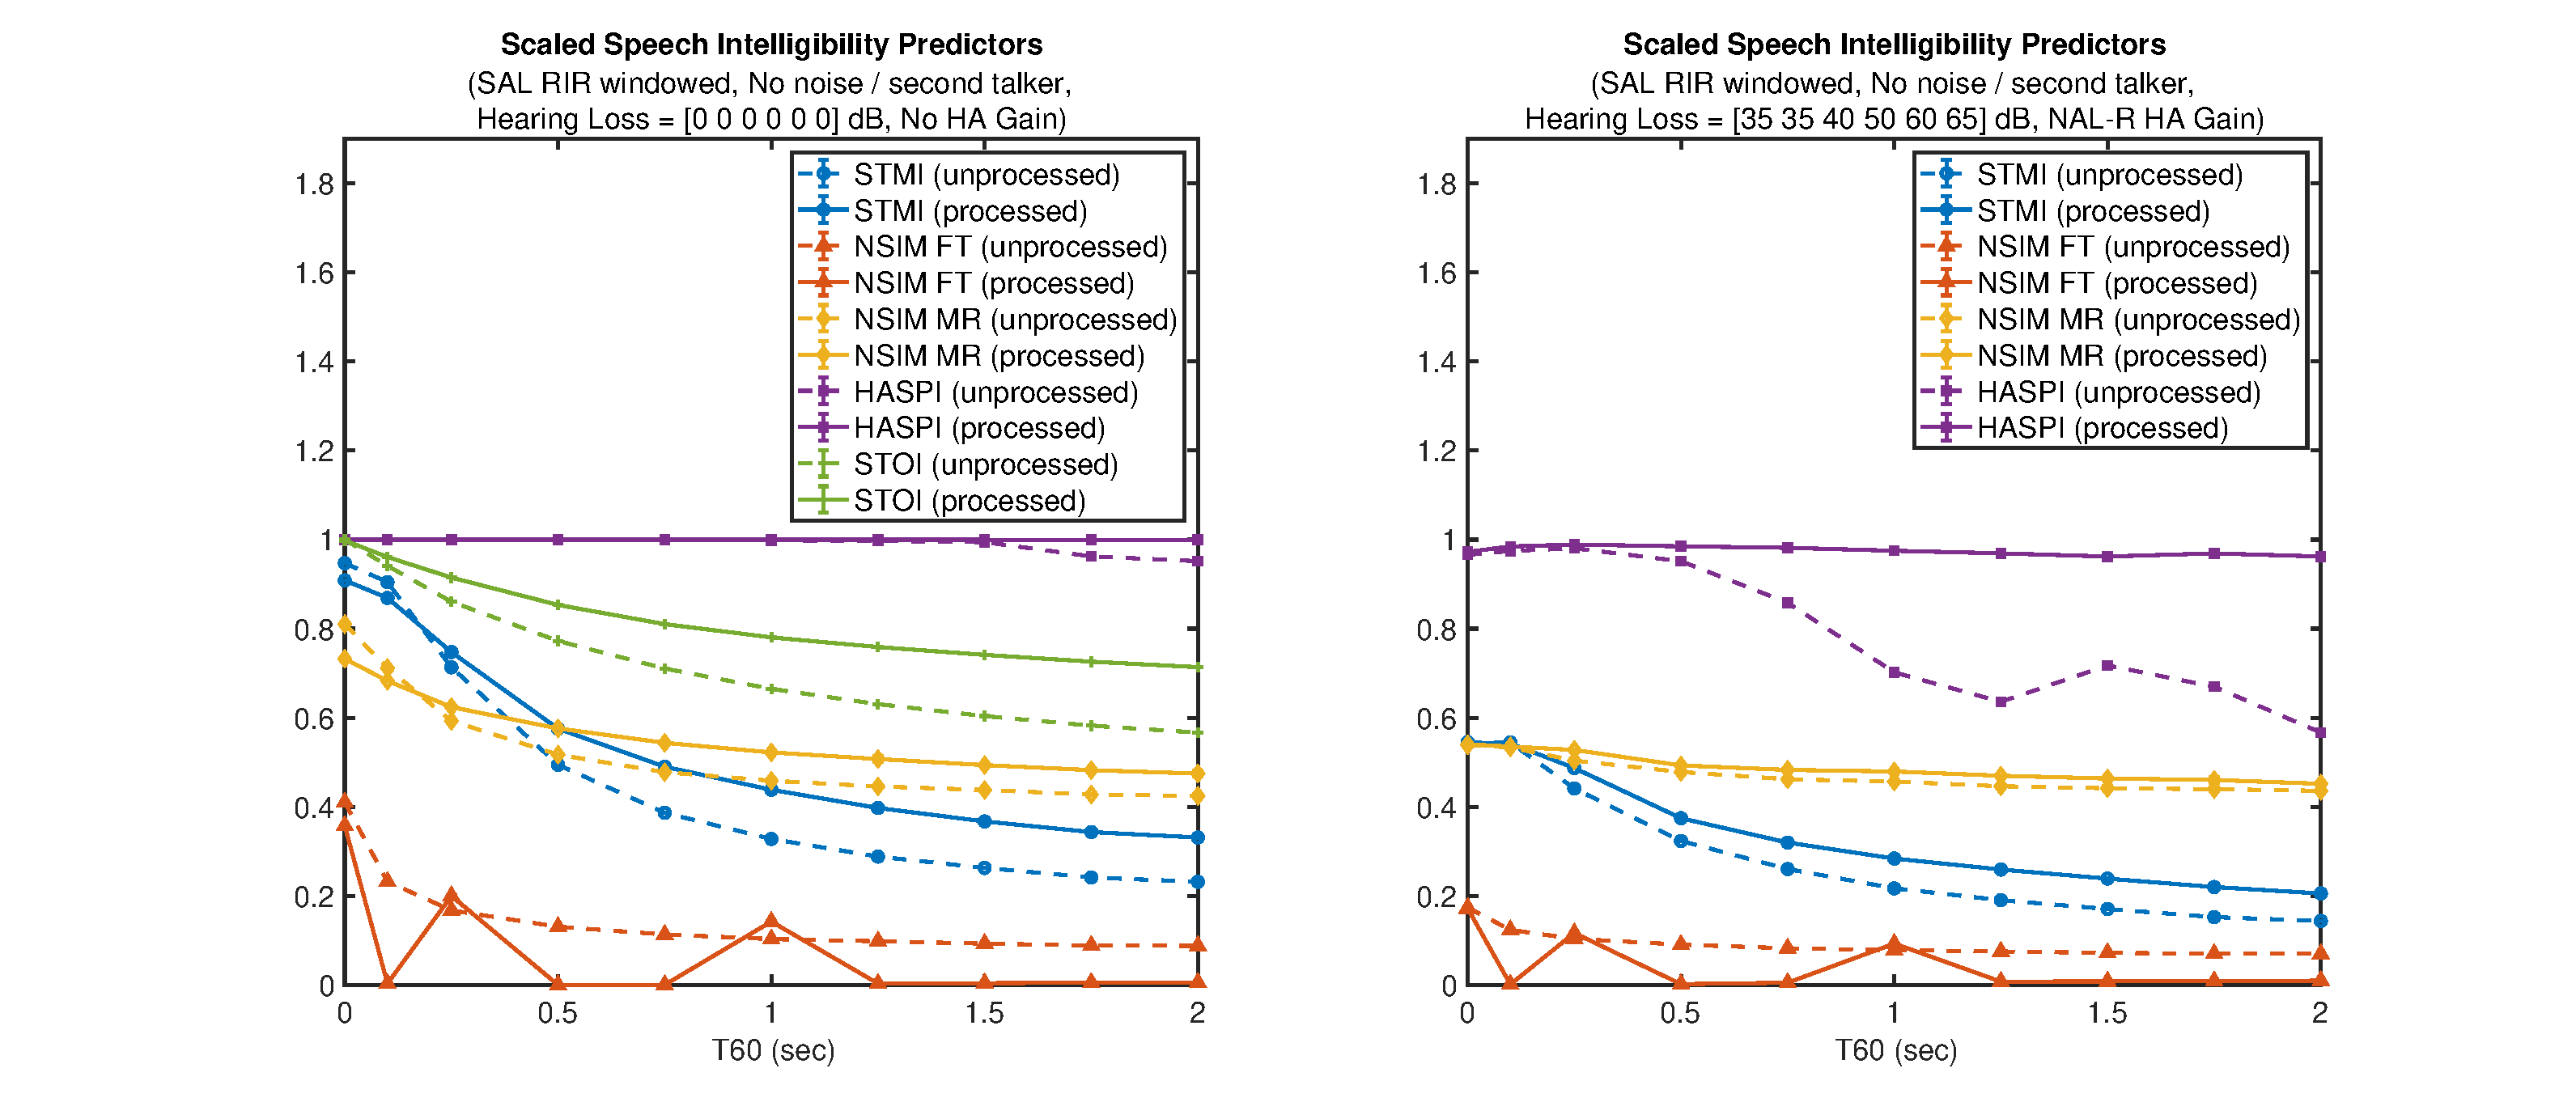
\includegraphics[width=\textwidth]{DAP_EVAL_1000T60max_wReg_SI_v_T60}
	\end{subfigure}
	\begin{subfigure}[b]{0.92\textwidth}
		\centering
		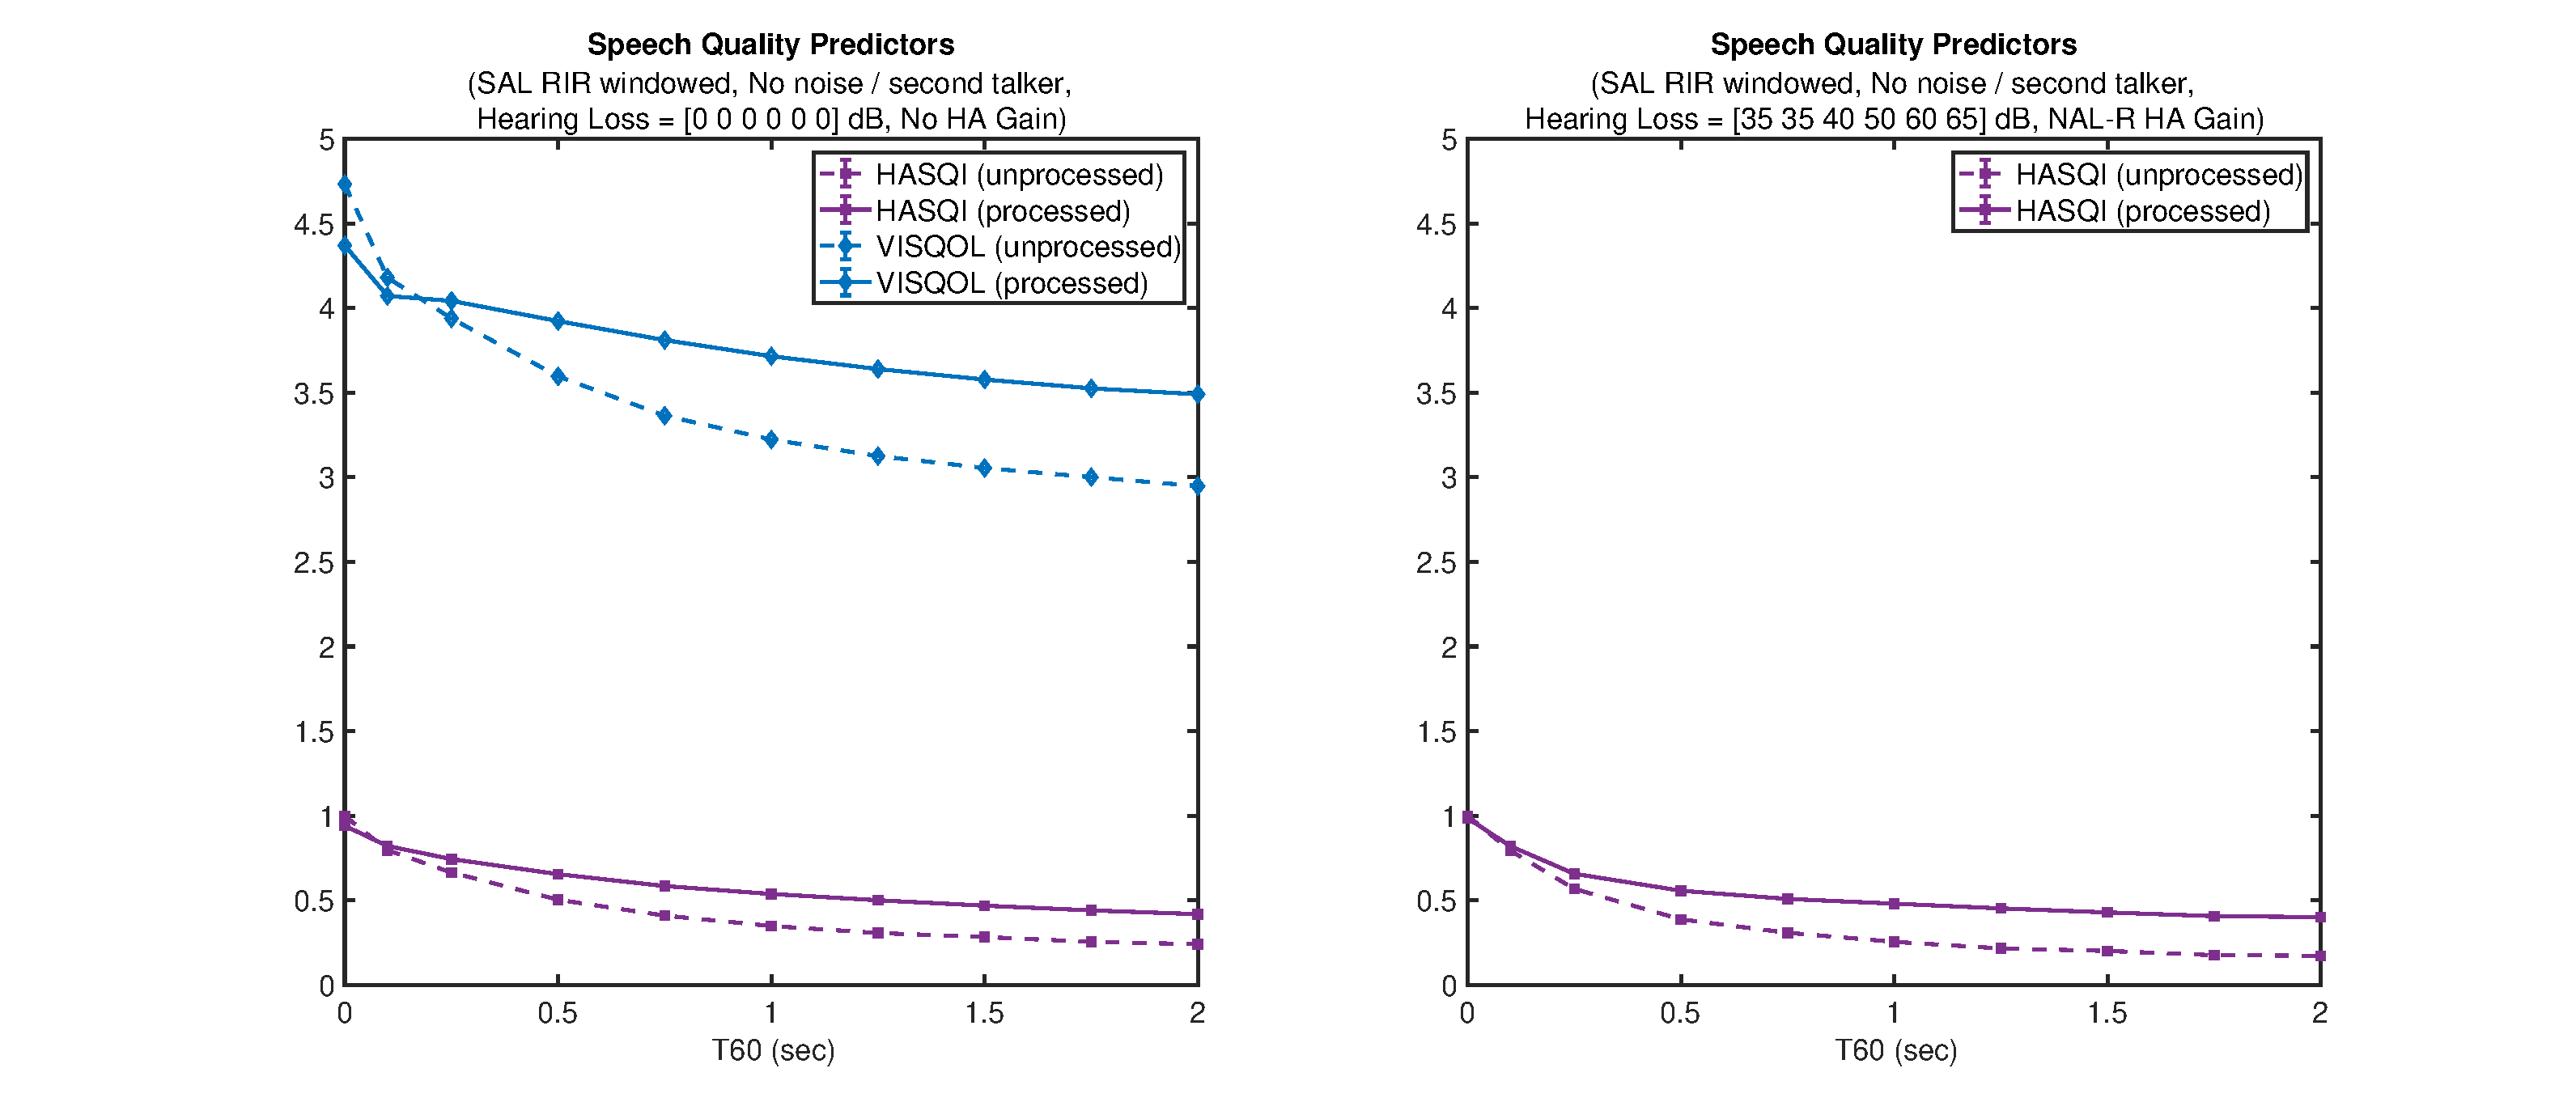
\includegraphics[width=\textwidth]{DAP_EVAL_1000T60max_wReg_SQ_v_T60}
	\end{subfigure}
	\caption[DAP evaluation with regularization and $p_2=2667$]{Evaluation of delay-and-predict dereverberation performance with autocorrelation regularization as a function of T60. Prediction orders were $p_2 = 5333$ and $p_1=20000$ (i.e., according to $T60_{\mathrm{max}} = \qty{1}{\sec}$ for$M=4$ and $f_s=\qty{16}{\kilo\hertz})$. RIRs were generated by applying a variable decay-rate exponential window to a measured RIR (The SAL room from the MYRiAD database, $\mathrm{T60} = \qty{2.2}{\second}$) to control T60. No Noise or Interfering talker were included.}
	\label{fig:DAP_EVAL_1000T60max_wReg}
\end{figure}



